\documentclass[final,3p,times,number]{elsarticle}
\usepackage[utf8]{inputenc}
\usepackage{graphicx}
\usepackage{booktabs}
\usepackage{array}
\usepackage{tabularx}
\usepackage{multirow}
\usepackage{amsmath}
\usepackage{amssymb}
\usepackage{placeins}
\usepackage{float}
\usepackage[font=small,skip=6pt]{caption}
\usepackage{subcaption}
\usepackage{microtype}
\usepackage{tikz}
\usepackage{url}
\usepackage{etoolbox}
\usepackage{iftex}
\ifXeTeX
  % XeTeX (tectonic) cannot use the 8-bit Times fonts loaded by the class option,
  % which leaves text without bold or italic; load OpenType Times/Helvetica clones.
  \usepackage{fontspec}
  \setmainfont{texgyretermes}[Extension=.otf, UprightFont=*-regular, BoldFont=*-bold,
    ItalicFont=*-italic, BoldItalicFont=*-bolditalic]
  \setsansfont{texgyreheros}[Extension=.otf, UprightFont=*-regular, BoldFont=*-bold,
    ItalicFont=*-italic, BoldItalicFont=*-bolditalic]
\fi
\usetikzlibrary{arrows.meta,positioning,shapes.geometric,calc,fit}
\urlstyle{same}
\captionsetup{labelfont=bf,justification=centering}
\emergencystretch=2em
\newcolumntype{Y}{>{\raggedright\arraybackslash}X}
\setlength{\textfloatsep}{12pt plus 2pt minus 3pt}
\setlength{\floatsep}{12pt plus 2pt minus 3pt}
\setlength{\intextsep}{12pt plus 2pt minus 3pt}
\renewcommand{\arraystretch}{1.08}
\raggedbottom
% visible gap between paragraphs
\setlength{\parskip}{6pt plus 1fil}
% never break a paragraph (and so never a sentence) across pages; a page may end
% short instead (unlimited bottom stretch), and a paragraph only splits if it
% cannot fit on a page at all
\makeatletter
\def\@textbottom{\vskip \z@ \@plus 1fill}
% the kernel re-inserts \interlinepenalty where a float was defined, which would
% make the gap between paragraphs around every float unbreakable; use 0 there
\patchcmd{\@specialoutput}{\addpenalty \interlinepenalty}{\addpenalty \z@}{}{\PatchFailed}
\patchcmd{\@addtocurcol}{\addpenalty \interlinepenalty}{\addpenalty \z@}{}{\PatchFailed}
\patchcmd{\@addtocurcol}{\penalty\interlinepenalty}{\penalty\z@}{}{\PatchFailed}
\makeatother
\AtBeginDocument{%
  \interlinepenalty=10000
  \clubpenalty=10000
  \widowpenalty=10000
  \displaywidowpenalty=10000
  \predisplaypenalty=10000
}
\setcounter{topnumber}{5}
\setcounter{bottomnumber}{2}
\setcounter{totalnumber}{6}
\renewcommand{\topfraction}{0.95}
\renewcommand{\bottomfraction}{0.85}
\renewcommand{\textfraction}{0.05}
\renewcommand{\floatpagefraction}{0.7}
\makeatletter
% start float-only pages at the top instead of centring them vertically
\setlength{\@fptop}{0pt}
\setlength{\@fpsep}{18pt plus 4pt}
\setlength{\@fpbot}{0pt plus 1fil}
\makeatother
\journal{Engineering Applications of Artificial Intelligence}

\begin{document}
\begin{frontmatter}

\title{Standardised Comparison of Convolutional and Transformer Backbones for Brain Tumour MRI Classification under Perceptual-Hash Deduplication}

\author[scope]{Parth Mital}
\author[scope]{Ved Lawand}
\author[scope]{Biji C. L.\corref{cor1}}
\author[sbst]{Muzaffar Ahamad Dar}
\author[sbst]{George Priya Doss C.}
\cortext[cor1]{Corresponding author. Email address: biji.cl@vit.ac.in}

\affiliation[scope]{organization={School of Computer Science and Engineering, Vellore Institute of Technology},
city={Vellore}, state={Tamil Nadu}, country={India}}
\affiliation[sbst]{organization={School of Bio Sciences and Technology, Vellore Institute of Technology},
city={Vellore}, state={Tamil Nadu}, country={India}}

\begin{abstract}
Magnetic resonance imaging (MRI) is the standard investigation for brain tumours, but manual interpretation is slow, variable between readers, and dependent on expertise that is unevenly distributed. Deep learning has been applied widely to this problem, yet reported accuracies are difficult to compare because studies differ in dataset, preprocessing, splitting and evaluation, and because near-duplicate images drawn from shared public sources frequently leak between training and test partitions. We benchmark nine ImageNet-pretrained backbones spanning classical convolutional networks (ResNet50, VGG16, DenseNet121), efficient convolutional networks (EfficientNetB0, MobileNetV3-Large, InceptionV3) and transformer or hybrid architectures (ViT-B/16, Swin-Base, CoAtNet-0) under matched data, preprocessing and schedule. Six of the nine were additionally evaluated on three-way subtype classification. Perceptual hashing applied before splitting removed 19.3\% near-duplicate images from the multiclass collection, reducing 5,828 MRI images to 4,705 unique samples; binary detection used a separate set of 3,253 images. All models were initialised from ImageNet weights and fine-tuned using the AdamW optimiser, a cosine annealing learning rate schedule, and mixed precision training on two NVIDIA Tesla T4 graphics processing units. On the held-out test set, CoAtNet-0, DenseNet121, EfficientNetB0, and ResNet50 each reached 99.39\% binary detection accuracy, with DenseNet121 and ResNet50 attaining an area under the receiver operating characteristic curve (AUC) of 1.0000. For multiclass classification, Swin-Base achieved the highest accuracy of 98.58\% with a macro-averaged one-versus-rest AUC of 0.9993, followed by CoAtNet-0 at 98.44\% and InceptionV3 at 98.30\%. EfficientNetB0 offered the best accuracy-to-cost balance, reaching 99.39\% detection accuracy and 97.59\% subtype accuracy with only 4.0 million parameters, 0.77 GFLOPs per image, and 10.8~ms single-image latency. Gradient-weighted class activation mapping indicates that the highest-accuracy subtype model attends substantially to regions outside the brain, so accuracy alone does not establish that pathology has been learned.
\end{abstract}

\begin{keyword}
Brain tumour MRI \sep deep learning \sep perceptual hashing \sep shortcut learning \sep vision transformers
\end{keyword}

\end{frontmatter}

\section{Introduction}
\label{sec:intro}

Brain tumours constitute the abnormal proliferation of cells either in the brain or the central nervous system. Whether benign or malignant, brain tumours represent serious threats because of their location in the limited skull cavity and the important functions of the brain. According to the Central Brain Tumor Registry of the United States, 453,623 primary brain and other central nervous system tumours were diagnosed in the United States between 2016 and 2020, an average of approximately 90,700 cases per year \cite{cbtrus}. The exact prevalence in India, however, is not fully documented. Three major forms of primary brain tumours include: (i) glioma, which is formed from glial cells and accounts for 26.3\% of all primary brain and other central nervous system tumours in the same registry \cite{cbtrus}; (ii) meningioma, which develops in the meningeal layers of the brain and is usually benign in nature; and (iii) pituitary tumours, which grow in the pituitary gland and cause hormonal problems \cite{ref2}.

Magnetic resonance imaging (MRI) is used nowadays as the main non-invasive technique for brain tumour detection and classification. In comparison to traditional computed tomography imaging, MRI gives much better soft tissue contrast without utilising any ionising radiation. Moreover, MRI allows images to be acquired in different orientations and with different types of contrast, namely T1-weighted, T2-weighted, fluid-attenuated inversion recovery (FLAIR), and diffusion-weighted. This is extremely important for determining tumour location, volume, margins, oedema, and adjacent vital structures. At the same time, analysis of MRI studies raises a number of problems that cannot be ignored. Firstly, examination takes a lot of time, because a complete brain MRI study may include hundreds of sections, each of which must be reviewed. Secondly, inter- and intra-observer variability should be noted, as there is no guarantee that radiologists will interpret the results of an MRI study in the same way. Thirdly, limited training in neuroradiology can become an obstacle to correct image interpretation. Finally, there are not enough specialists in the rural and semi-urban regions of India because of the poor radiologist-to-population ratio.

The introduction of deep learning technology has transformed the field of medical imaging analysis in the last ten years. Models based on deep learning, especially convolutional neural networks (CNNs), have the ability to learn hierarchical representations of visual features directly from pixel inputs without the need for manual feature extraction. Thus, the use of these models enables automatic, efficient, and consistent tumour detection from brain MRI images. Convolutional neural networks have become popular among researchers working in this area, with well-performing models such as ResNet, VGG, DenseNet, Inception, EfficientNet, and MobileNet setting benchmarks on image classification tasks. More recently, researchers started exploring transformer models for computer vision problems, having been introduced initially for natural language processing. These transformer-based models include the vision transformer (ViT), the Swin Transformer, and CoAtNet. This line of research provides an alternative way of representing global information in images using the self-attention mechanism, and it might be of particular use in medical imaging, especially for understanding the relation between a tumour and the surrounding anatomical structures \cite{ref28,ref29,ref30,ref32}.

Although several research works have separately proved the efficiency of deep learning architectures for detecting and classifying brain tumours, there is still an insufficient number of comparative investigations performed across several architectural families using the same experimental settings. The lack of comparative analysis poses serious challenges in choosing a suitable model, since each study employs a separate database, preprocessing procedure, data augmentation approach, and assessment technique, which makes it problematic to compare results reported by different studies. For example, it is impossible to say which performance figure is better when one work reports an accuracy of 99\% on a small and homogeneous database, whereas another gives 97\% accuracy on a larger and heterogeneous one.

Numerous papers make the mistake of retaining images that are duplicates or near-duplicates across the training, validation, and test splits when using publicly available datasets drawn from multiple sources. This results in a highly inaccurate assessment of performance, causing a significant increase in reported performance figures compared with the actual ability of a model to generalise. Once a model has been shown a particular image, or one that is very similar, during training, any further performance result for that image reflects memorisation rather than genuine learning. The problem of near-duplicate images is especially critical within brain tumour research, since most publicly available datasets come from common origins such as the Cheng dataset or the Figshare collection. Perceptual hashing addresses images that are duplicates of one another. It does not address a second and distinct form of correlation: adjacent slices of the same patient are visually different enough to survive any hash-based filter, yet are not statistically independent, so a split drawn at slice level can place highly correlated images on both sides of the partition even when no near-duplicate pair remains.

It is important to emphasise the clinical significance of establishing a brain tumour diagnosis correctly. The potential consequences of late diagnosis or misdiagnosis include limited treatment alternatives, poor prognosis, higher healthcare expenditure, and significantly diminished quality of life for both patients and their families. The implementation of automated systems with accuracy equal or superior to that of humans may bring about several advantages: faster diagnosis through prompt preliminary assessment; decision-making support where experienced radiologists are unavailable; uniformity of diagnosis due to the absence of inter-reader variation; and relief of radiologist workload so that experts attend primarily to challenging cases \cite{ref13,ref14}.

This paper makes four contributions. First, it establishes a matched-data, matched-preprocessing comparison of nine ImageNet-pretrained backbones spanning three architectural families on brain tumour MRI, and reports the optimisation budget each model actually received so that architecture and training budget can be separated by the reader. Second, it applies perceptual-hash deduplication before partitioning to both experimental tracks, quantifies the near-duplicate burden of the combined public collections, and reports how sensitive the resulting accuracies are to the deduplication threshold. Third, it reports the quantities that determine whether a model is deployable but are routinely omitted in this literature (per-class sensitivity and specificity, expected calibration error, agreement corrected for chance, and measured latency and throughput), and shows that models with identical accuracy differ in whether their errors are missed tumours or false alarms. Fourth, it audits whether the highest-accuracy model attends to pathology, and finds evidence that it does not, which constrains how the leaderboard should be interpreted.

The rest of this paper is structured as follows. Section~\ref{sec:lit} reviews existing studies on brain tumour classification. Section~\ref{sec:methods} describes the complete methodology adopted in this study, including the overall workflow, data collection, preprocessing, model development, and experimental settings. Section~\ref{sec:results} presents and discusses the results of both the binary detection and the multiclass classification tasks, together with efficiency and interpretability analyses. Section~\ref{sec:conclusion} concludes the study and offers directions for future research. Per-class tables, complete efficiency and training tables, and per-model figures are provided in the Supplementary Material, cited as Supplementary Tables S4--S10 and Figures S1--S16.

\section{Literature Review}
\label{sec:lit}

Previous works on automated brain tumour recognition were based on feature engineering followed by machine learning classifiers. Such works have used texture descriptors such as the grey level co-occurrence matrix (GLCM) and local binary patterns (LBP), wavelet transforms such as the discrete wavelet transform (DWT), morphological features related to shape, size, and boundary, and classifiers such as the support vector machine (SVM), random forests, and $k$-nearest neighbours \cite{ref2,ref3}. In their work, Zacharaki et al. \cite{ref1} obtained around 85\% accuracy using texture features and an SVM classifier on a small set of 80 images for tumour type recognition. Cheng et al. \cite{ref5} suggested a tumour region augmentation approach that yielded 90\% accuracy using intensity, texture, and shape features along with an SVM classifier on 3,064 MRI images. Although promising, such methods faced challenges due to the limitations of feature engineering, the inability to generalise across datasets, and the absence of automatic learning of hierarchical structures.

The success of AlexNet in 2012 propelled the implementation of deep learning in medical imaging applications. Successive CNN models improved performance by introducing better architectures. He et al. \cite{ref6} incorporated residual connections into CNN models, making it possible to train very deep networks by addressing the vanishing gradient problem. ResNet50 became a standard model for medical image classification, with reports of 95--98\% accuracy for brain tumour classification. Using transfer learning on a ResNet50 model, Seetha and Raja \cite{ref12} achieved an accuracy of 97.5\% for the classification of 253 brain MRI images. Simonyan and Zisserman \cite{ref4} demonstrated improvements in model performance by increasing depth while keeping small convolutional filters of size $3\times 3$. However, due to its very large parameter count of 138 million, VGG16 is computationally intensive and vulnerable to overfitting when applied to small medical datasets. For instance, Khan et al. \cite{ref23} reported 98.69\% accuracy using VGG16 with 3,064 samples. Huang et al. \cite{ref9} introduced densely connected layers in which each layer receives input from all preceding layers. Consequently, DenseNet121 became more parameter-efficient while achieving better performance in medical imaging tasks, with accuracies of 96--98\%. Szegedy et al. \cite{ref7} presented parallel convolutions with varying kernel dimensions ($1\times 1$, $3\times 3$, $5\times 5$) that allowed the model to learn multi-scale features. InceptionV3 reached 97.5\% accuracy in brain tumour classification, as reported by Deepak and Ameer \cite{ref15}. Moreover, Rehman et al. \cite{ref25} obtained a high classification rate of 99.34\% accuracy via transfer learning. Tan and Le \cite{ref18} introduced a method for scaling network dimensions, namely depth, width, and resolution, using neural architecture search to obtain better accuracy with far fewer parameters than comparable models. Furthermore, Howard et al. \cite{ref19} created lightweight neural networks based on depth-wise separable convolutions for mobile and edge devices.

Dosovitskiy et al. \cite{ref28} adapted transformer models to visual tasks by framing images as sequences of patches of $16\times 16$ pixels. The ViT-B/16 variant performed comparably with CNNs on large-scale datasets such as ImageNet and JFT-300M but needed extensive pre-training and exhibited drawbacks on small medical datasets because of a lack of built-in inductive biases. Liu et al. \cite{ref29} proposed hierarchical transformers using shifted windows to process images efficiently at multiple scales while retaining linear complexity with respect to image resolution. Swin Transformers performed impressively on ImageNet and have also been investigated for medical image processing. The hierarchical window attention in Swin Transformers enables the model to learn both local tumour boundaries and overall structure from MRI images. CoAtNet, proposed by Dai et al. \cite{ref30}, stacks depth-wise convolution stages and relative self-attention stages vertically within a single model, which is intended to combine the inductive bias of convolution with the global receptive field of attention.

Since 2022 these architectures have been applied to brain tumour MRI directly, and the reliability of the public benchmarks on which they are evaluated has itself come under scrutiny. Shamshad et al. \cite{shamshad2023} survey the adoption of transformers across medical imaging tasks, including classification. Tummala et al. \cite{tummala2022} fine-tuned an ensemble of four ImageNet-pretrained ViT variants on the 3,064-image Cheng collection and reported 98.7\% test accuracy for three-way subtype classification, and Asiri et al. \cite{asiri2024} reported 97\% accuracy for a Swin Transformer on a 2,870-image four-class Kaggle collection. Over the same period, Kapoor and Narayanan \cite{kapoor2023} documented data leakage, including leakage between training and test data, as a recurring cause of over-optimistic results in machine-learning-based science across 17 fields. Most directly relevant here, Vangala et al. \cite{vangala2026} audited public brain tumour MRI classification benchmarks and found that 28.8\% of the official test images of one widely used collection have a near-duplicate in its training split, and that 22.3\% of the test images of the Bhuvaji collection used in the present study are byte-identical to a training image. These findings strengthen the case for deduplicating before splitting rather than relying on the official partitions.

Studies applying these architectures to brain tumour detection and classification are summarised in Table~\ref{tab:existing-studies}.

\begin{table}[htbp]
\centering
\caption{Comparison of existing studies for brain tumour detection.}
\label{tab:existing-studies}
\small
\begin{tabular*}{\textwidth}{@{\extracolsep{\fill}}llccc@{}}
\toprule
Study & Model & Dataset size & Task & Accuracy \\
\midrule
Talo et al. (2019) \cite{ref16} & ResNet50 & 253 & Binary & 95.23\% \\
Khan et al. (2020) \cite{ref23} & VGG16 & 3,064 & Binary & 98.69\% \\
Noreen et al. (2020) \cite{ref24} & DenseNet121 & 3,064 & Binary & 99.51\% \\
Rehman et al. (2020) \cite{ref25} & InceptionV3 & 3,064 & Binary & 99.34\% \\
Ghassemi et al. (2020) \cite{ref26} & EfficientNet & 3,064 & Binary & 98.87\% \\
Cheng et al. (2015) \cite{ref5} & SVM + features & 3,064 & Multiclass & 90.00\% \\
Deepak and Ameer (2019) \cite{ref15} & InceptionV3 & 3,064 & Multiclass & 97.50\% \\
Tummala et al. (2022) \cite{tummala2022} & ViT ensemble & 3,064 & Multiclass & 98.70\% \\
Asiri et al. (2024) \cite{asiri2024} & Swin Transformer & 2,870 & Multiclass & 97.00\% \\
\bottomrule
\end{tabular*}
\end{table}

Several open issues remain. Cross-architecture comparison is difficult because most studies examine no more than two or three models. Dataset heterogeneity is a further obstacle, because split schemes, preprocessing, and evaluation protocols differ between studies. Transformer under-representation is an additional problem, since current papers deal mainly with CNN-based models. Reproducibility is also limited, because source code, exact splits, and pretrained weights are not consistently released. Incomplete deduplication is a final gap, as most papers do not account for duplicate and near-duplicate images in combined datasets. Reporting practice is also narrow: headline accuracy and AUC are commonly quoted without per-class sensitivity and specificity, without any assessment of probability calibration, and without measured inference cost, all of which matter for clinical interpretation. This paper addresses these gaps by evaluating nine architectures under identical conditions, combining datasets from multiple public sources, applying perceptual hash based deduplication before splitting, comparing CNN and transformer families directly, reporting per-class and calibration metrics alongside measured latency and throughput, and releasing the complete code and per-model artefacts for both the binary and the multiclass tasks.

\section{Methods and Materials}
\label{sec:methods}

\subsection{Overall Methodology}
\label{sec:workflow}

The complete research workflow adopted in this study is illustrated in Figure~\ref{fig:methodology}. The pipeline proceeds through five stages. In the data acquisition stage, two publicly available Kaggle collections are combined for the binary detection task and two further collections are combined for the multiclass subtype task. In the data curation stage, perceptual hashing is applied to the multiclass collection to remove near-duplicate images before any split is drawn, after which both datasets are partitioned into training, validation, and test subsets using stratified sampling so that class proportions are preserved in every subset. In the preprocessing stage, images are converted to three-channel form, resized to the input resolution expected by each backbone, normalised using ImageNet statistics, and augmented on the fly during training only. In the model development stage, nine ImageNet-pretrained backbones are fine-tuned under a single shared training protocol, with the classification head of each backbone replaced to match the number of target classes. In the evaluation stage, the checkpoint selected on the validation split is applied once to the held-out test split, and accuracy, per-class sensitivity and specificity, F1 score, AUC, calibration error, gradient-weighted class activation maps, and inference cost are recorded for every model.

A design point worth stating explicitly is that the two tasks are kept separate rather than merged into a single four-class problem. The binary detector answers whether a tumour-like abnormality is present, whereas subtype classification is only meaningful once a tumour-positive decision has already been taken. Keeping the tasks separate mirrors the clinical order of interpretation and avoids making the subtype model responsible for rejecting tumour-negative images that were never part of its training objective.

\begin{figure*}[htbp]
\centering
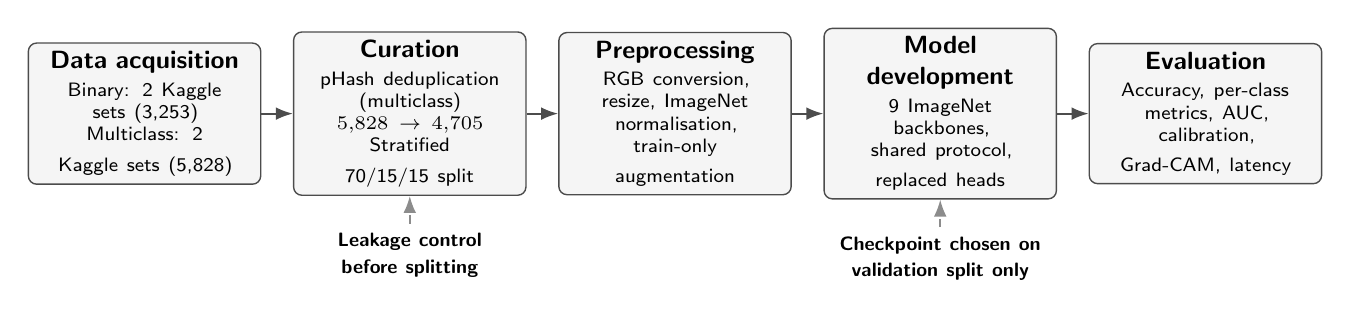
\begin{tikzpicture}[
  font=\sffamily\small,
  >=Latex,
  stage/.style={draw=black!70, fill=black!4, rounded corners=3pt, line width=0.5pt,
                text width=2.74cm, align=center, minimum height=1.55cm, inner sep=3pt},
  lbl/.style={font=\sffamily\bfseries\footnotesize},
  arrow/.style={->, line width=0.7pt, draw=black!70}
]
\node[stage] (acq) {\textbf{Data acquisition}\\[2pt]\scriptsize Binary: 2 Kaggle\\ sets (3,253)\\ Multiclass: 2\\ Kaggle sets (5,828)};
\node[stage, right=0.4cm of acq] (cur) {\textbf{Curation}\\[2pt]\scriptsize pHash deduplication\\ (multiclass)\\ $5{,}828\rightarrow4{,}705$\\ Stratified\\ 70/15/15 split};
\node[stage, right=0.4cm of cur] (pre) {\textbf{Preprocessing}\\[2pt]\scriptsize RGB conversion,\\ resize, ImageNet\\ normalisation,\\ train-only\\ augmentation};
\node[stage, right=0.4cm of pre] (mod) {\textbf{Model}\\\textbf{development}\\[2pt]\scriptsize 9 ImageNet\\ backbones,\\ shared protocol,\\ replaced heads};
\node[stage, right=0.4cm of mod] (ev) {\textbf{Evaluation}\\[2pt]\scriptsize Accuracy, per-class\\ metrics, AUC,\\ calibration,\\ Grad-CAM, latency};

\draw[arrow] (acq) -- (cur);
\draw[arrow] (cur) -- (pre);
\draw[arrow] (pre) -- (mod);
\draw[arrow] (mod) -- (ev);

\node[below=0.35cm of cur, lbl, text width=3.2cm, align=center] (t1)
  {\scriptsize Leakage control before splitting};
\node[below=0.35cm of mod, lbl, text width=3.2cm, align=center] (t2)
  {\scriptsize Checkpoint chosen on validation split only};
\draw[arrow, dashed, draw=black!45] (t1) -- (cur);
\draw[arrow, dashed, draw=black!45] (t2) -- (mod);
\end{tikzpicture}
\caption{Overall methodology of the study, showing the five stages of the pipeline from data acquisition through curation, preprocessing, and model development to evaluation. Perceptual hash deduplication is applied before splitting so that near-duplicate images cannot leak between training and test subsets, and the test split is used only once, with the checkpoint selected on the validation split.}
\label{fig:methodology}
\end{figure*}

\subsection{Data Collection}
\label{sec:data}

For the binary brain tumour detection task, which requires classifying MRI images as either tumour-positive or tumour-negative, we combined two publicly available brain MRI datasets sourced from the Kaggle platform. Dataset~1, \textit{Brain MRI Images for Brain Tumor Detection} \cite{ds1}, contains 253 MRI images in total, with 155 labelled as tumour-positive and 98 as tumour-negative. Dataset~2, \textit{Br35H: Brain Tumor Detection 2020} \cite{ds2}, contains a substantially larger collection of 3,000 MRI images with a perfectly balanced distribution of 1,500 tumour-positive and 1,500 tumour-negative images. The images are provided in JPEG format and have been pre-cropped to focus on the brain region, though some variability in field of view and image resolution exists across samples. The combined dataset for binary classification comprised 3,253 images, with 1,598 tumour-negative images (49.1\%) and 1,655 tumour-positive images (50.9\%). This near-perfect balance prevents the model from exploiting class imbalance and keeps chance-level accuracy at approximately 50\%. The negative class consists of images that the dataset curators labelled as not containing a tumour; neither source certifies that these images are radiologically normal, so the absence of other pathology is not established, and the class is accordingly referred to as tumour-negative rather than normal throughout. Representative samples of tumour-negative and tumour-positive images are shown in Figure~\ref{fig:binary-samples}, and the class distribution is given in Supplementary Figure~S3.

For the more challenging multiclass classification task, in which the model must distinguish between glioma, meningioma, and pituitary tumours, we combined two further publicly available brain tumour MRI datasets. Dataset~1, Bhuvaji et al., \textit{Brain Tumor Classification (MRI)} \cite{ds3}, provides JPEG images at variable native resolution; its training and testing folders were merged, and its tumour-negative folder was excluded because the multiclass task contains tumour classes only. Dataset~2 is the brain tumour collection of Cheng et al. \cite{ds4}, described in the associated study \cite{ref5}, which comprises 3,064 contrast-enhanced T1-weighted slices of $512\times 512$ pixels from 233 patients, and was obtained in the JPEG conversion distributed on Kaggle \cite{ds5}. The Bhuvaji collection is widely understood to be derived in substantial part from the Cheng data. The combined dataset prior to deduplication consisted of 5,828 images, with glioma the largest subset at 2,352 images (40.4\%), meningioma at 1,645 images (28.2\%), and pituitary at 1,831 images (31.4\%). Representative samples of each tumour type are shown in Figure~\ref{fig:cls-samples}.

The provenance of every image is summarised in Table~\ref{tab:provenance}, which gives for each source the number of images contributed, the class-by-source contingency, the native resolution, and the recorded MRI sequence. The Cheng counts are those of the source publication; the Bhuvaji counts are the per-class totals of the pooled collection less the Cheng counts. The deduplication pass described in Section~\ref{sec:preproc} recorded only per-class totals, so the number of images from each source that survived deduplication, and the division of the 1,123 removed images into cross-source and within-source duplicates, were not recorded and cannot be reported from these runs.

The MRI sequence is unknown in both experimental tracks. Neither binary source records the sequence (T1-weighted, contrast-enhanced T1-weighted, T2-weighted, or FLAIR) of individual images. In the multiclass track, the Cheng component is contrast-enhanced T1-weighted according to its source publication \cite{ref5}, but the Bhuvaji collection records no sequence information, so the pooled multiclass set is a mixture of unknown sequence composition. This limits clinical interpretation: a model trained on an unknown mixture of sequences cannot be specified for deployment on any particular acquisition protocol.

\begin{table*}[htbp]
\centering
\caption{Provenance of the source collections before deduplication, giving the images contributed by each source, the class-by-source contingency, the native resolution, and the recorded MRI sequence. Bhuvaji counts cover the merged training and testing folders of the three tumour classes. Per-source counts surviving deduplication were not recorded by the deduplication pass (Section~\ref{sec:preproc}).}
\label{tab:provenance}
\small
\setlength{\tabcolsep}{4pt}
\begin{tabular*}{\textwidth}{@{\extracolsep{\fill}}llccccll@{}}
\toprule
Track & Source & Images & \multicolumn{3}{c}{Class counts} & Native resolution & Sequence \\
\midrule
 & & & Tumour & Tumour-negative & & & \\
\cmidrule(lr){4-5}
\multirow{3}{*}{Binary} & Chakrabarty \cite{ds1} & 253 & 155 & 98 & & Variable$^{a}$ & Not recorded \\
 & Br35H \cite{ds2} & 3,000 & 1,500 & 1,500 & & Variable$^{a}$ & Not recorded \\
 & \textbf{Total} & \textbf{3,253} & \textbf{1,655} & \textbf{1,598} & & & \\
\midrule
 & & & Glioma & Meningioma & Pituitary & & \\
\cmidrule(lr){4-6}
\multirow{3}{*}{Multiclass} & Bhuvaji \cite{ds3} & 2,764 & 926 & 937 & 901 & Variable$^{a}$ & Not recorded \\
 & Cheng \cite{ds4,ds5} & 3,064 & 1,426 & 708 & 930 & $512\times 512$ & Contrast-enhanced T1 \\
 & \textbf{Total} & \textbf{5,828} & \textbf{2,352} & \textbf{1,645} & \textbf{1,831} & & \\
\bottomrule
\multicolumn{8}{@{}l}{\footnotesize $^{a}$Per-source dimension statistics were not computed; pooled statistics for each track are given in Table~\ref{tab:image-dims}.}
\end{tabular*}
\end{table*}

The two collections differ substantially in their native image geometry, as summarised in Table~\ref{tab:image-dims} and illustrated in Supplementary Figures~S1 and S2. The binary detection images are heterogeneous, with widths ranging from 150 to 1,920 pixels and a standard deviation of 155 to 195 pixels about mean dimensions of roughly 300 to 400 pixels, reflecting the varied cropping and field of view of the two contributing sources. The multiclass images are far more uniform, with a median of $512\times 512$ pixels in every class and interquartile ranges that collapse to a single value, since the great majority of images were distributed at that resolution. This difference matters for interpretation: the multiclass task operates on a visually homogeneous collection, whereas the binary task requires the model to absorb considerably more variation in scale and framing. All images were resized to a common input resolution during preprocessing, so this heterogeneity affects the effective magnification of anatomy rather than the tensor shape presented to the network.

\begin{table}[htbp]
\centering
\caption{Native image dimensions of the source collections before resizing, in pixels. Values are computed across all images of each class prior to deduplication.}
\label{tab:image-dims}
\small
\begin{tabular*}{\textwidth}{@{\extracolsep{\fill}}llcccccc@{}}
\toprule
Task & Class & Images & Mean W & Mean H & SD W & Min W & Max W \\
\midrule
\multirow{2}{*}{Binary} & No tumour & 1,598 & 302.6 & 308.9 & 154.9 & 150 & 1,920 \\
 & Tumour & 1,655 & 351.5 & 400.2 & 195.2 & 175 & 1,275 \\
\midrule
\multirow{3}{*}{Multiclass} & Glioma & 2,352 & 507.6 & 508.4 & 33.0 & 175 & 640 \\
 & Meningioma & 1,645 & 483.1 & 485.9 & 90.4 & 174 & 1,275 \\
 & Pituitary & 1,831 & 512.5 & 512.2 & 84.4 & 201 & 1,365 \\
\bottomrule
\end{tabular*}
\end{table}

\begin{figure}[htbp]
\centering
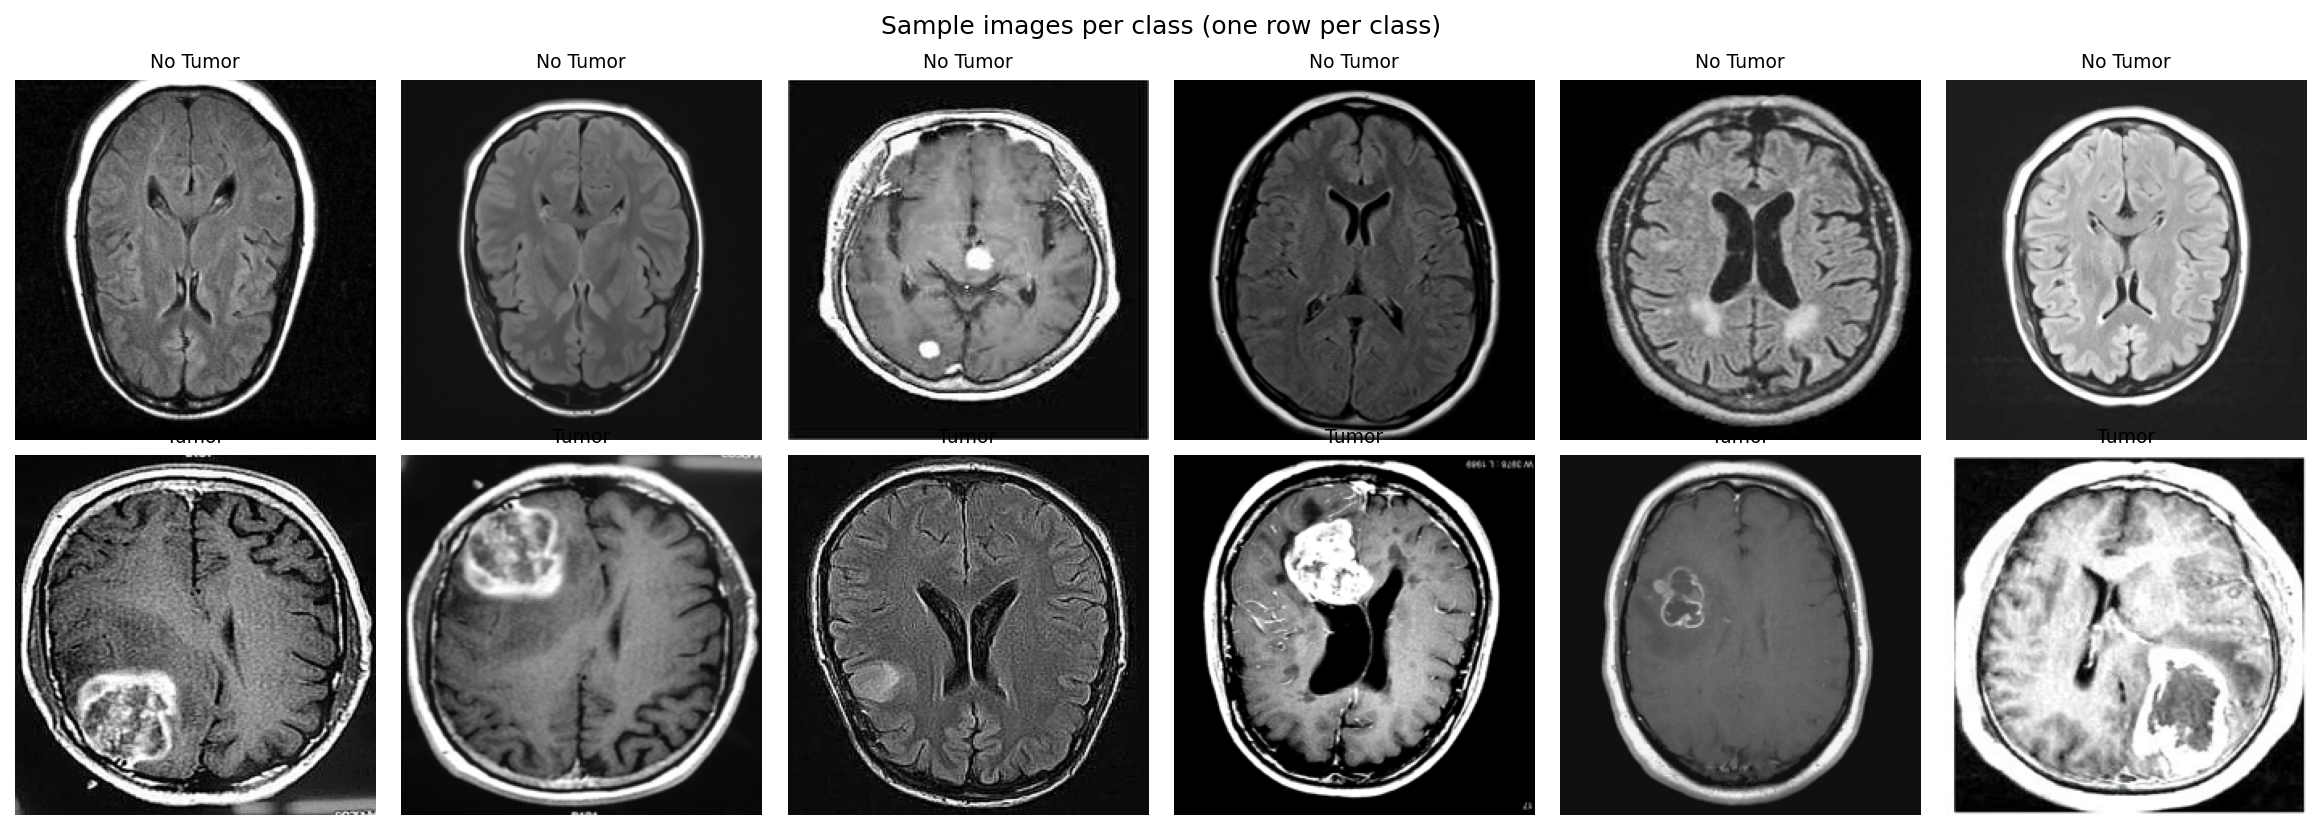
\includegraphics[width=\linewidth]{figures/binary_samples.png}
\caption{Sample brain MRI images used for the binary detection task. The top row shows tumour-negative images and the bottom row shows tumour-positive images.}
\label{fig:binary-samples}
\end{figure}

\begin{figure}[htbp]
\centering
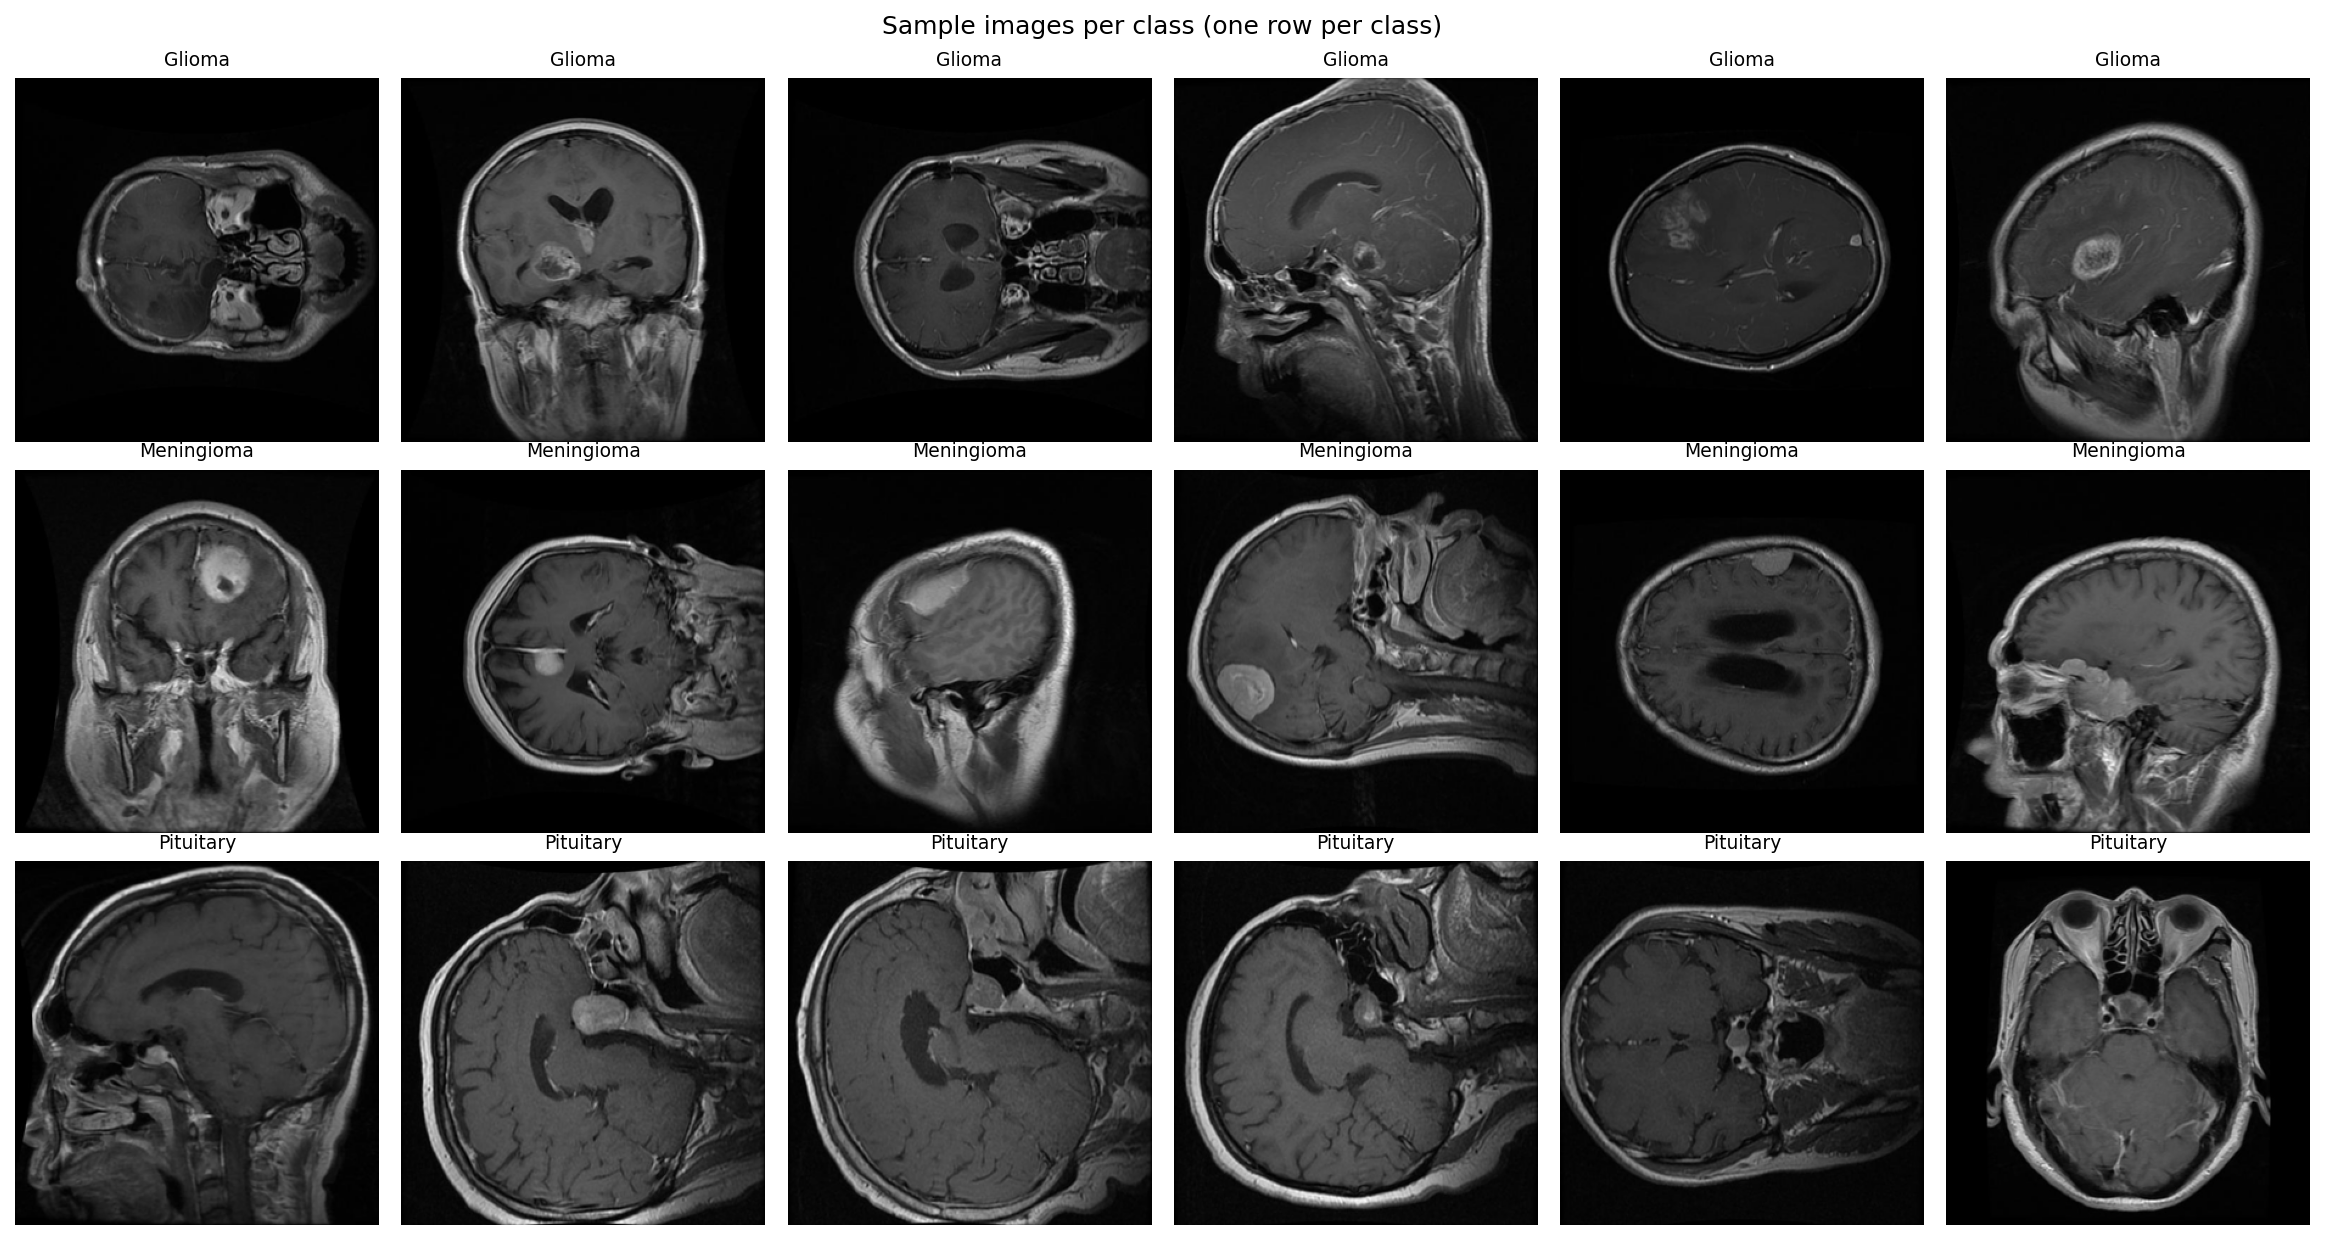
\includegraphics[width=\linewidth]{figures/cls_samples.png}
\caption{Sample MRI images by tumour type for the multiclass classification task, showing glioma, meningioma, and pituitary cases.}
\label{fig:cls-samples}
\end{figure}

\subsection{Preprocessing and Deduplication}
\label{sec:preproc}

When working with multiple datasets there is always a possibility of encountering duplicates, or images of the same underlying content that differ only in resizing or compression. These near-duplicates, if inadvertently distributed across training and test splits, constitute a form of data leakage that artificially inflates reported performance. To address this, we employed perceptual hashing (pHash), which generates a compact fingerprint for each image that is robust to resizing, compression, slight rotation, and minor contrast adjustment. Specifically, 64-bit perceptual hashes were generated using the ImageHash library. The Hamming distance between two hash values served as the similarity metric. We adopted a tolerance threshold of 5, so that any pair of images differing in at most 5 of the 64 bits was treated as a near-duplicate pair, and all but one representative of each such group were removed. The rationale for rigorous deduplication is that multiple public datasets often contain the same underlying images because they derive from common original sources, that near-duplicates cause leakage if present across train and test splits, and that removal of duplicates ensures reported metrics reflect genuine generalisation.

Deduplication was applied to the multiclass collection, where the two constituent datasets are known to overlap substantially. After applying perceptual hashing, the glioma class decreased from 2,352 to 2,000 images, a reduction of 14.97\%; meningioma decreased from 1,645 to 1,304 images, a reduction of 20.73\%; and pituitary decreased from 1,831 to 1,401 images, a reduction of 23.48\%. Overall, the multiclass dataset was reduced from 5,828 to 4,705 images, a reduction of 19.3\%. The class distribution before and after deduplication is shown in Figure~\ref{fig:dedup}.

It should be stated explicitly that perceptual hash deduplication was \emph{not} applied to the binary detection dataset. The two binary source collections are disjoint in origin and the smaller of the two contributes only 253 of the 3,253 images, so the risk of cross-dataset duplication was judged to be low. This is nevertheless an asymmetry between the two experimental tracks: the multiclass results are protected against near-duplicate leakage by construction, whereas the binary results are not, and the binary figures reported in Section~\ref{sec:binary-results} should be read with that caveat in mind. Applying the same deduplication procedure to the binary track is identified in Section~\ref{sec:conclusion} as a priority for future work.

\begin{figure}[htbp]
\centering
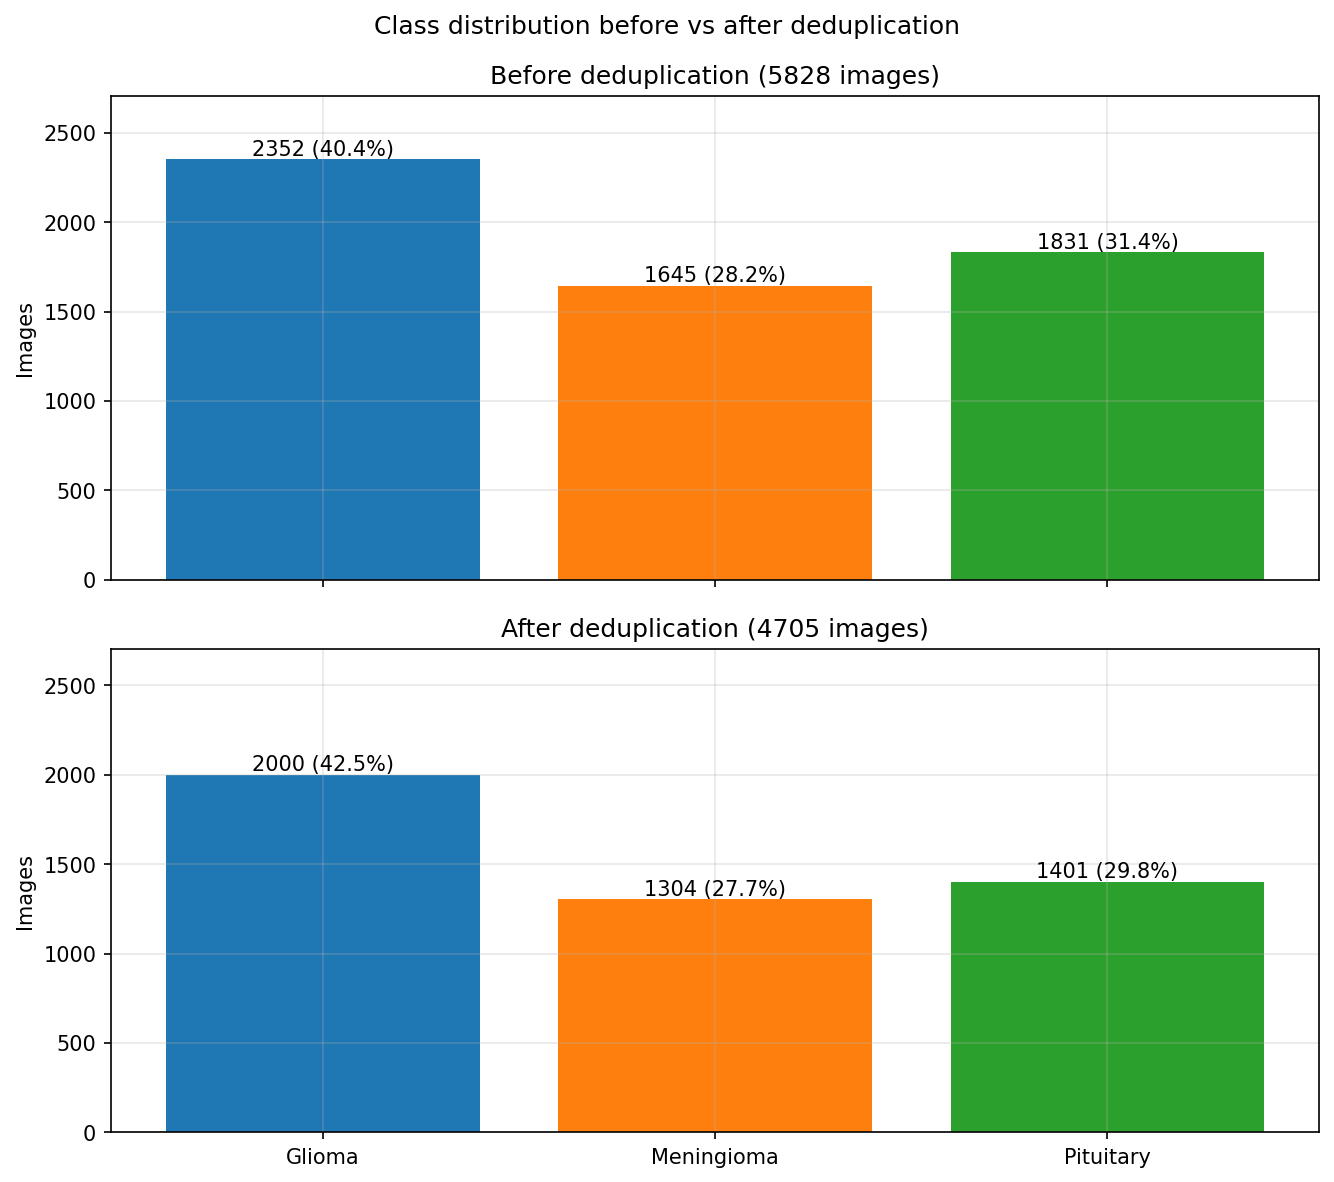
\includegraphics[width=\linewidth]{figures/cls_deduplication.png}
\caption{Class distribution of the multiclass dataset before and after perceptual hash deduplication. The total decreased from 5,828 to 4,705 images, a reduction of 19.3\%.}
\label{fig:dedup}
\end{figure}

Stratified sampling was used for both splits so that every subset retained a representative distribution of the classes. For binary detection, the 3,253 images were divided into training, validation, and test subsets in the proportions 70\%, 15\%, and 15\%, giving 2,277, 488, and 488 images respectively. For multiclass classification, the same proportions were applied to the 4,705 deduplicated images, giving 3,293 training, 706 validation, and 706 test images. The resulting per-class split sizes are reported in Table~\ref{tab:splits}.

\begin{table}[htbp]
\centering
\caption{Stratified dataset splits for both tasks. Proportions are 70\% training, 15\% validation, and 15\% test in each case.}
\label{tab:splits}
\small
\begin{tabular*}{\textwidth}{@{\extracolsep{\fill}}llccc@{}}
\toprule
Task & Class & Training & Validation & Test \\
\midrule
\multirow{3}{*}{Binary detection} & No tumour & 1,119 & 239 & 240 \\
 & Tumour & 1,158 & 249 & 248 \\
 & \textbf{Total} & \textbf{2,277} & \textbf{488} & \textbf{488} \\
\midrule
\multirow{4}{*}{Multiclass} & Glioma & 1,400 & 300 & 300 \\
 & Meningioma & 913 & 195 & 196 \\
 & Pituitary & 980 & 211 & 210 \\
 & \textbf{Total} & \textbf{3,293} & \textbf{706} & \textbf{706} \\
\bottomrule
\end{tabular*}
\end{table}

All images were loaded using the Python Imaging Library and converted to the RGB colour format even where the original was greyscale, ensuring compatibility with the ImageNet-pretrained backbones. Images were resized to the input resolution expected by each backbone, which was $224\times 224$ pixels for every model except InceptionV3, which requires $299\times 299$ pixels. Pixel values were converted to a PyTorch tensor and scaled to the range $[0,1]$, then normalised using the ImageNet channel means of $[0.485, 0.456, 0.406]$ and standard deviations of $[0.229, 0.224, 0.225]$. To improve generalisation, data augmentation was applied exclusively to the training set and consisted of random horizontal flipping with probability 0.5, random rotation of up to $\pm 10$ degrees, and colour jitter adjusting brightness and contrast by up to 20\%. These augmentations were applied on the fly at each epoch. For validation and testing, only resizing, tensor conversion, and normalisation were applied, with no stochastic augmentation, ensuring deterministic and reproducible evaluation. Representative images before and after augmentation for both tasks are shown in Supplementary Figure~S6.

\subsection{Model Development}
\label{sec:models}

Nine architectures spanning three families were evaluated. All were initialised from ImageNet-pretrained weights, and in every case the final classification layer was replaced with a linear layer producing one output for the binary task or three outputs for the multiclass task. The parameter counts quoted below and used throughout the paper are the counts measured directly from the instantiated models after head replacement, and therefore differ slightly from the nominal counts commonly quoted for the ImageNet-1000 variants of the same backbones. These measured values are reported consistently in Tables~\ref{tab:binary-results}, \ref{tab:multiclass-results}, and \ref{tab:efficiency}.

ResNet50 is a 50-layer residual network built around bottleneck residual blocks with skip connections that address the vanishing gradient problem, measured at 23.51 million parameters. VGG16 is a 16-layer network using only $3\times 3$ convolutional filters stacked in increasing depth, measured at 134.26 million parameters. DenseNet121 is a 121-layer densely connected network that concatenates the feature maps of all preceding layers, maximising information flow at only 6.95 million parameters. EfficientNetB0, developed through neural architecture search and compound scaling, achieves strong accuracy with only 4.01 million parameters and 0.77 GFLOPs per image. MobileNetV3-Large uses depth-wise separable convolutions for mobile and embedded applications, measured at 4.20 million parameters and the lowest computational cost in the study at 0.43 GFLOPs per image. InceptionV3 is a 48-layer network with parallel convolutional paths of different kernel sizes within inception modules, capturing multi-scale features at 24.35 million parameters and operating at the higher input resolution of $299\times 299$ pixels. ViT-B/16 divides the input image into $16\times 16$ patches and processes them as a sequence with a transformer encoder, measured at 85.80 million parameters and lacking the convolutional inductive bias of the CNN backbones. Swin-Base introduces hierarchical transformers with shifted windows, achieving linear complexity and multi-scale processing at 86.74 million parameters. CoAtNet-0 combines convolutional and attention mechanisms in a unified architecture and is measured at 26.67 million parameters. We note that CoAtNet-0 is frequently described in the literature as a model of approximately 10 million parameters; the implementation used here is the \texttt{coatnet\_0\_rw\_224} variant, whose measured size is 26.67 million parameters, and that measured value is what is reported throughout.

The multiclass track was run for six of the nine architectures, namely CoAtNet-0, EfficientNetB0, InceptionV3, ResNet50, Swin-Base, and ViT-B/16. VGG16, DenseNet121, and MobileNetV3-Large were evaluated on the binary detection task only.

\subsection{Training Configuration}
\label{sec:training}

All experiments were conducted on dual NVIDIA Tesla T4 graphics processing units with 16~GB of GDDR6 memory each, Intel Xeon processors with four virtual central processing unit cores, and 29~GB of system memory, running Python 3.12.13 with PyTorch 2.10.0 and CUDA 12.8. To ensure fair comparison, the hyperparameters listed in Table~\ref{tab:hyperparams} were standardised across all models. Every model was trained for 10 epochs using the AdamW optimiser, which is the Adam optimiser with decoupled weight decay regularisation, at an initial learning rate of $3\times 10^{-4}$ and the library default weight decay coefficient of 0.01, which was left unchanged rather than tuned. The learning rate was annealed using the cosine annealing learning rate scheduler with the maximum number of iterations parameter set to 10, matching the number of epochs, so that the learning rate followed a single cosine decay from its initial value to approximately zero over the course of training. The loss function was binary cross-entropy with logits loss for the binary detection task, which combines a sigmoid activation with the binary cross-entropy criterion in a numerically stable form, and cross-entropy loss for the multiclass task. Mixed precision training was used throughout, with automatic mixed precision autocasting and gradient scaling to preserve numerical stability in half precision.

Batch sizes were model-specific and set to the largest value that fitted within the available graphics memory, since a single batch size would have been infeasible for the largest transformer backbones. The batch sizes used are listed per model in Supplementary Tables~S9 and S10. This has an important consequence that must be stated plainly: because the learning rate and epoch count are held fixed while the batch size varies from 32 to 256, the number of optimiser steps each model receives varies correspondingly, from roughly 80 to 350 over the ten epochs. The comparison is therefore controlled for data, schedule, and preprocessing, but it is \emph{not} controlled for optimisation budget, and a model trained at batch size 256 receives far fewer gradient updates than one trained at batch size 64. Differences between models consequently confound architecture with optimisation budget to an extent that cannot be separated from these runs alone.

The training loader used \texttt{drop\_last=True}, so any final partial batch was discarded at each epoch. At batch size 256 this means 2,048 of the 2,277 binary training images were used per epoch, with 229 images dropped; because the loader reshuffles, the dropped subset differs from epoch to epoch, so all images are seen over the course of training but no single epoch sees the full set. The training loop at each epoch consisted of a training phase with augmentation and weight updates followed by a validation phase without augmentation. Learning rate scheduling was applied after each epoch. Model checkpointing retained the weights giving the best validation AUC for the binary task and the best validation macro AUC for the multiclass task, with the first epoch attaining the maximum retained.

The random seed was fixed at 42 for PyTorch, NumPy, and the Python standard library random module. Reproducibility is nevertheless only approximate rather than exact, because \texttt{cudnn.benchmark} was enabled, TF32 matrix multiplication was permitted, and automatic mixed precision was used throughout; each of these admits non-deterministic kernel selection. Re-running a notebook should reproduce the reported figures closely but not necessarily bit-for-bit.

\begin{table}[htbp]
\centering
\caption{Training hyperparameters, standardised across all models and both tasks.}
\label{tab:hyperparams}
\small
\begin{tabularx}{\textwidth}{@{}lY@{}}
\toprule
Hyperparameter & Setting \\
\midrule
Epochs & 10 \\
Optimiser & AdamW (Adam with decoupled weight decay) \\
Weight decay & 0.01 \\
Initial learning rate & $3\times 10^{-4}$ \\
Learning rate scheduler & Cosine annealing, maximum iterations $=10$ \\
Loss (binary detection) & Binary cross-entropy with logits loss \\
Loss (multiclass) & Cross-entropy loss \\
Precision & Mixed precision with automatic casting and gradient scaling \\
Batch size & Model-specific; largest fitting in memory (see Supplementary Tables~S9 and S10) \\
Input resolution & $224\times 224$ pixels; $299\times 299$ pixels for InceptionV3 \\
Checkpoint selection & Best validation AUC (binary), best validation macro one-versus-rest AUC (multiclass); first epoch attaining the maximum \\
Random seed & 42 \\
\bottomrule
\end{tabularx}
\end{table}

\subsection{Implementation Differences Between Models}
\label{sec:impl}

Each architecture was implemented in its own notebook from a shared template, and the intended difference between notebooks is the backbone alone. In practice a small number of further differences were necessary or arose incidentally, and since several of them bear on the interpretation of the results they are documented here rather than left implicit. They are summarised in Table~\ref{tab:impl-diffs}.

Two differences are unavoidable. First, each architecture exposes its classification head under a different attribute, so the head replacement code necessarily differs. Second, the layer targeted for gradient-weighted class activation mapping must be the last spatial or token stage of each architecture, which differs by design; for VGG16 this resolves to a max-pooling rather than a convolutional layer, which makes its attention maps less directly comparable with the others.

One difference is an inconsistency that should be taken into account when reading the two tasks together. Most backbones were obtained from \texttt{torchvision}; CoAtNet-0 was obtained from \texttt{timm} in both tasks, since CoAtNet has no \texttt{torchvision} implementation. Swin-Base, however, was not sourced consistently: the binary detection notebook uses the \texttt{timm} model \texttt{swin\_base\_patch4\_window7\_224}, whereas the multiclass notebook uses the \texttt{torchvision} model \texttt{swin\_b}. These are different implementations of the Swin-B architecture and they load different pretrained checkpoints, so the two rows labelled Swin-Base in Tables~\ref{tab:binary-results} and \ref{tab:multiclass-results} are not the same model initialised the same way. Their measured parameter counts differ only marginally, at 86.74 and 86.75 million, but the comparison of Swin-Base across the two tasks is not strictly like-for-like, and the contrast between its weak binary result of 95.90\% and its leading multiclass result of 98.58\% should not be attributed to task difficulty alone.

Two differences affect results and deserve particular attention. The InceptionV3 binary notebook applies the standard auxiliary-classifier recipe, adding $0.4$ times the auxiliary loss to the main loss during training, which no other model receives. Separately, although the InceptionV3 binary model is wrapped for two-GPU data parallelism, the training loop calls the unwrapped module, so the run executed on a single GPU; the recorded peak memory of 0~MB on the second device confirms this. Its training time in Supplementary Table~S9 is therefore a single-GPU measurement and is not comparable with the other rows, a point returned to in Section~\ref{sec:efficiency}. In the multiclass InceptionV3 notebook the auxiliary head is disabled but not removed, so 769,000 parameters belonging to an unused 1000-class auxiliary classifier remain in the model and are counted in its reported total of 25.12~million. This accounts for the difference between the binary and multiclass InceptionV3 parameter counts in Tables~\ref{tab:binary-results} and \ref{tab:multiclass-results}, and it is the reason those two figures are not identical despite the backbone being the same.

\begin{table*}[htbp]
\centering
\caption{Implementation differences between the per-model notebooks, with the reason for each. Differences confined to comments, cell titles, or equivalent reformatting are not listed.}
\label{tab:impl-diffs}
\small
\begin{tabularx}{\textwidth}{@{}llY@{}}
\toprule
Difference & Scope & Reason \\
\midrule
Head replacement code & All models & Each architecture exposes its classifier under a different attribute; unavoidable. \\
Source library \texttt{timm} & CoAtNet-0 (both tasks) & CoAtNet has no \texttt{torchvision} implementation. \\
Source library differs \emph{between tasks} & Swin-Base & \texttt{timm} \texttt{swin\_base\_patch4\_window7\_224} for binary, \texttt{torchvision} \texttt{swin\_b} for multiclass. Different implementations and different pretrained checkpoints; no stated reason. \\
Input resolution $299\times 299$ & InceptionV3 & The architecture's native input size. \\
Batch size (32--256) & All models & Set to the largest value fitting in 16~GB of graphics memory. Only InceptionV3 states this in code; for the others it is inferred from recorded peak memory. Changes the optimisation budget. \\
Auxiliary loss $0.4\times$ & InceptionV3 (binary) & Standard Inception training recipe; applied without comment. \\
Single-GPU execution & InceptionV3 (binary) & The training loop calls the unwrapped module, bypassing data parallelism. Unintended. \\
Retained unused auxiliary head & InceptionV3 (multiclass) & Only the main head was replaced; adds 769k parameters to the reported total. Unintended. \\
Grad-CAM target layer & All models & Must be the final spatial or token stage of each architecture. For VGG16 this is a max-pooling layer. \\
Pinned \texttt{IMAGENET1K\_V1} weights & MobileNetV3-Large & The only model not using the library default weights. No stated reason. \\
\bottomrule
\end{tabularx}
\end{table*}

A further asymmetry concerns the deduplication procedure itself. The perceptual hash pass operates over the combined multiclass pool without regard to class label, and processes classes in a fixed order, so where a near-duplicate pair spans two classes the glioma image is always the one retained. Such cross-label removals are neither counted nor reported by the procedure. The class-wise reduction percentages in Section~\ref{sec:preproc} should therefore be read as the outcome of an order-dependent process rather than as an intrinsic measure of redundancy within each class.

Finally, the multiclass source collection was assembled by merging the official training and testing folders of the Bhuvaji dataset into a single pool before applying deduplication and drawing new stratified splits. This was done so that both tasks would use the same 70/15/15 splitting procedure, but it means the multiclass results are not directly comparable with published figures that evaluate on that dataset's original test split, a point returned to in Section~\ref{sec:comparison}.

\section{Results and Discussion}
\label{sec:results}

This section presents the findings of the binary detection and multiclass classification experiments. Section~\ref{sec:binary-results} reports binary tumour detection, Section~\ref{sec:multiclass-results} reports classification into glioma, meningioma, and pituitary subtypes, Section~\ref{sec:efficiency} compares computational efficiency, Section~\ref{sec:interpretability} examines model interpretability through gradient-weighted class activation mapping, and Section~\ref{sec:comparison} compares the present results with previously published work. Unless stated otherwise, every figure quoted is measured on the held-out test split.

\subsection{Binary Detection Results}
\label{sec:binary-results}

Test-split results for the binary detection task are reported in Table~\ref{tab:binary-results}, and the per-class breakdown for every model is given in Supplementary Table~S4. Four architectures tied at the highest accuracy of 99.39\%, corresponding to three misclassified images out of 488: CoAtNet-0, DenseNet121, EfficientNetB0, and ResNet50. Although the accuracy of these four models is identical, the structure of their errors differs in a way that matters clinically. CoAtNet-0 and EfficientNetB0 achieved perfect sensitivity of 100.00\% at a specificity of 98.75\%, so every tumour-positive test image was detected and the three errors were false alarms on tumour-negative images, whereas DenseNet121 and ResNet50 showed the mirror-image behaviour, achieving perfect specificity of 100.00\% at a sensitivity of 98.79\%, so their three errors were missed tumours. Figure~\ref{fig:binary-confusion} shows this contrast directly for EfficientNetB0 and ResNet50. For a screening application in which a missed tumour is the more serious failure, the error profile of CoAtNet-0 and EfficientNetB0 is preferable despite the identical headline accuracy, although DenseNet121 and ResNet50 produced the strongest threshold-independent ranking, both reaching an AUC of 1.0000 to four decimal places. The four leaders should nevertheless be regarded as statistically indistinguishable rather than genuinely tied: on a test set of 488 images a single misclassification is worth 0.20 percentage points of accuracy, each model was trained once from a single seed, no confidence intervals are available, and the separation between the four leaders and InceptionV3 amounts to three images. The top of Table~\ref{tab:binary-results} therefore identifies a group of models that perform equivalently on this data rather than ordering them, whereas the distinction between that group and the weaker models spans tens of images and is not in doubt.

InceptionV3 followed at 98.77\% accuracy with an AUC of 0.9986. The three transformer and hybrid models diverged sharply: CoAtNet-0, which combines convolution with attention, matched the best CNNs, whereas the two pure transformers trailed, with Swin-Base at 95.90\% and ViT-B/16 at 94.88\%. MobileNetV3-Large reached only 90.78\% accuracy despite an AUC of 0.9981, and this gap between ranking quality and accuracy is diagnostic of a badly placed decision threshold rather than poor discrimination: its sensitivity was 81.85\% against a specificity of 100.00\%, its expected calibration error of 0.0685 was the worst in the study, and its optimal Youden threshold of 0.00044 lies some three orders of magnitude below the 0.5 decision point actually used, so that 45 tumours are missed purely through threshold placement and recalibration alone would recover most of the loss. Its validation loss of 0.3995 against a training accuracy of 99.90\% at the final epoch indicates substantial overfitting. VGG16 performed worst at 88.32\% accuracy with an AUC of 0.9676, consistent with the expectation that a 134-million-parameter architecture without residual or dense connectivity is poorly suited to a dataset of this size. Training and validation curves, receiver operating characteristic and precision--recall curves, and reliability diagrams for all nine binary models are given in Supplementary Figures~S7, S9, and S11, and the per-class metric summary, representative predictions, and validation and row-normalised confusion panels of EfficientNetB0 in Supplementary Figures~S12, S13, and S14.

\begin{table*}[htbp]
\centering
\caption{Binary detection results on the held-out test split (488 images). Sensitivity is recall of the tumour-positive class and specificity is recall of the tumour-negative class. Parameter counts are measured from the instantiated models. Rows are ordered by accuracy.}
\label{tab:binary-results}
\small
\begin{tabular*}{\textwidth}{@{\extracolsep{\fill}}lccccccc@{}}
\toprule
Model & Acc. (\%) & Sens. (\%) & Spec. (\%) & F1 (\%) & AUC & Test loss & Params (M) \\
\midrule
CoAtNet-0 & 99.39 & 100.00 & 98.75 & 99.40 & 0.9999 & 0.0253 & 26.67 \\
DenseNet121 & 99.39 & 98.79 & 100.00 & 99.39 & 1.0000 & 0.0189 & 6.95 \\
EfficientNetB0 & 99.39 & 100.00 & 98.75 & 99.40 & 0.9998 & 0.0233 & 4.01 \\
ResNet50 & 99.39 & 98.79 & 100.00 & 99.39 & 1.0000 & 0.0217 & 23.51 \\
InceptionV3 & 98.77 & 97.98 & 99.58 & 98.78 & 0.9986 & 0.0419 & 24.35 \\
Swin-Base & 95.90 & 93.55 & 98.33 & 95.87 & 0.9961 & 0.1117 & 86.74 \\
ViT-B/16 & 94.88 & 96.37 & 93.33 & 95.03 & 0.9862 & 0.1525 & 85.80 \\
MobileNetV3-Large & 90.78 & 81.85 & 100.00 & 90.02 & 0.9981 & 0.3698 & 4.20 \\
VGG16 & 88.32 & 86.29 & 90.42 & 88.25 & 0.9676 & 0.2448 & 134.26 \\
\bottomrule
\end{tabular*}
\end{table*}

\begin{figure}[htbp]
\centering
\begin{subfigure}{0.49\linewidth}
\centering
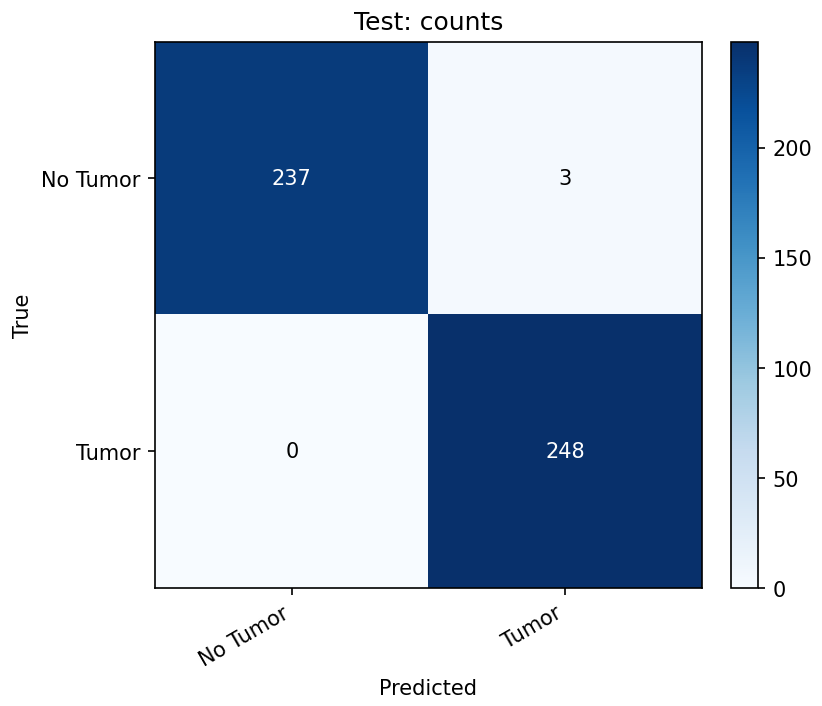
\includegraphics[width=\linewidth]{figures/binary_confusion_test.png}
\caption{EfficientNetB0.}
\end{subfigure}
\hfill
\begin{subfigure}{0.49\linewidth}
\centering
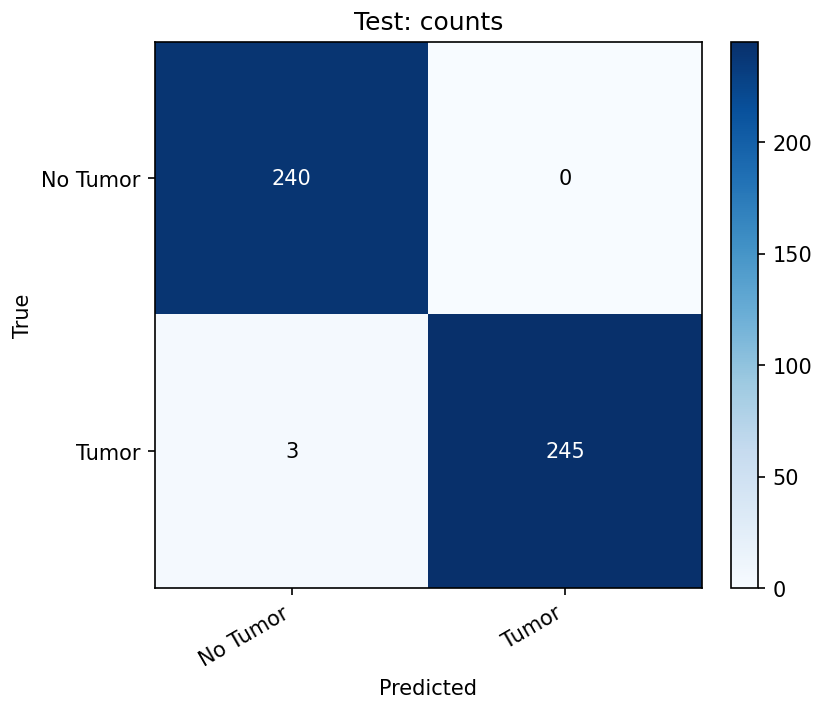
\includegraphics[width=\linewidth]{figures/binary_resnet_confusion_test.png}
\caption{ResNet50.}
\end{subfigure}
\caption{Test-split confusion matrices for \textbf{EfficientNetB0} and \textbf{ResNet50} on the binary detection task, both at 99.39\% accuracy. The three EfficientNetB0 errors are false positives on tumour-negative images, whereas the three ResNet50 errors are missed tumours. Validation and row-normalised panels are given in Supplementary Figure~S14.}
\label{fig:binary-confusion}
\end{figure}

\subsection{Multiclass Classification Results}
\label{sec:multiclass-results}

Test-split results for classification into glioma, meningioma, and pituitary subtypes are reported in Table~\ref{tab:multiclass-results}, and the per-class breakdown in Supplementary Table~S5. Swin-Base achieved the highest accuracy at 98.58\%, corresponding to 10 misclassified images out of 706, with a balanced accuracy of 98.42\%, a macro F1 score of 98.47\%, and the lowest test loss in the study at 0.0410. CoAtNet-0 followed at 98.44\% and InceptionV3 at 98.30\%, the latter achieving the highest macro one-versus-rest AUC at 0.9994. EfficientNetB0 and ResNet50 tied at 97.59\% accuracy, which is notable given that EfficientNetB0 uses 4.01 million parameters against 23.51 million for ResNet50, a difference of almost six times for identical accuracy. ViT-B/16 was again the weakest model by a substantial margin at 90.51\% accuracy and a macro AUC of 0.9759. Meningioma is consistently the hardest class: Swin-Base, CoAtNet-0, and EfficientNetB0 all reached a meningioma sensitivity of 95.92\%, well below their glioma and pituitary sensitivities, and meningioma carries the lowest F1 score for five of the six models. This is clinically plausible, since meningiomas arise from the meningeal layers and can present with less distinctive intensity and shape signatures on a single two-dimensional slice than the typically well-localised pituitary lesions, and meningioma is also the smallest class, with 913 training images against 1,400 for glioma. The test-split confusion matrices confirm the pattern: of the 10 Swin-Base errors in Figure~\ref{fig:cls-swin-confusion}, 8 are meningioma cases assigned to another class and no pituitary case is misclassified, while EfficientNetB0 in Figure~\ref{fig:cls-confusion} makes 17 errors on the same 706 images, seven more for a twenty-onefold reduction in parameter count.

The contrast between Swin-Base and ViT-B/16 is the clearest architectural signal in these results. Both are transformer backbones of almost identical size, 86.75 million and 85.80 million parameters respectively, yet they differ by just over eight percentage points in accuracy. Swin-Base imposes a hierarchical, locally windowed attention structure that reintroduces a spatial inductive bias, whereas ViT-B/16 treats the image as a flat sequence of patches and must learn that structure from data; with only 3,293 training images there is insufficient data to learn it, and the pure transformer underperforms. CoAtNet-0 supports the same reading from the other direction, reaching 98.44\% by combining convolutional stages with attention stages at under a third of the parameters of either pure transformer. The conclusion is not that attention is unhelpful for this task but that, at this data scale, attention needs to be paired with a convolutional prior. This reading should be qualified by the interpretability evidence in Section~\ref{sec:interpretability}, which indicates that part of the Swin-Base advantage may rest on non-anatomical image cues; the architectural argument and the shortcut explanation are not mutually exclusive, and these experiments cannot separate them. Training curves for all six multiclass models are given in Supplementary Figure~S8, their one-versus-rest receiver operating characteristic and precision--recall curves in Supplementary Figure~S10 and reliability diagrams in Supplementary Figure~S11, and the per-class metric summary, representative predictions, and validation and row-normalised confusion panels of EfficientNetB0 in Supplementary Figures~S12, S13, and S14.

\begin{table*}[htbp]
\centering
\caption{Multiclass classification results on the held-out test split (706 images). Precision and F1 are macro-averaged across the three tumour classes, and AUC is the macro-averaged one-versus-rest value. Rows are ordered by accuracy.}
\label{tab:multiclass-results}
\small
\begin{tabular*}{\textwidth}{@{\extracolsep{\fill}}lccccccc@{}}
\toprule
Model & Acc. (\%) & Bal. acc. (\%) & Prec. (\%) & F1 (\%) & AUC & Test loss & Params (M) \\
\midrule
Swin-Base & 98.58 & 98.42 & 98.54 & 98.47 & 0.9993 & 0.0410 & 86.75 \\
CoAtNet-0 & 98.44 & 98.21 & 98.50 & 98.35 & 0.9989 & 0.0521 & 26.67 \\
InceptionV3 & 98.30 & 98.29 & 98.17 & 98.22 & 0.9994 & 0.0471 & 25.12 \\
EfficientNetB0 & 97.59 & 97.50 & 97.41 & 97.45 & 0.9988 & 0.0588 & 4.01 \\
ResNet50 & 97.59 & 97.57 & 97.36 & 97.46 & 0.9988 & 0.0593 & 23.51 \\
ViT-B/16 & 90.51 & 90.37 & 90.31 & 90.34 & 0.9759 & 0.2637 & 85.80 \\
\bottomrule
\end{tabular*}
\end{table*}

\begin{figure}[htbp]
\centering
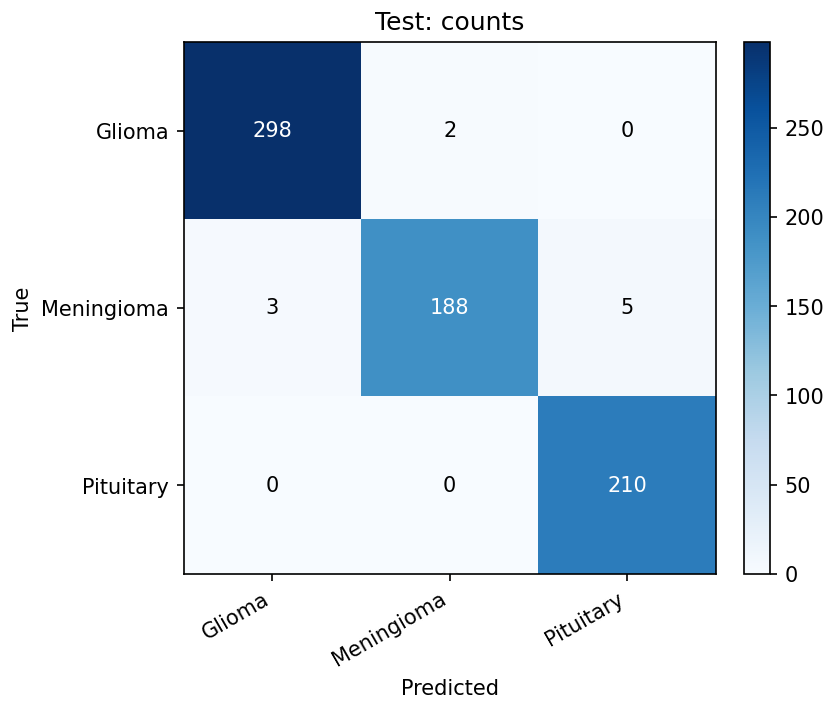
\includegraphics[width=0.62\linewidth]{figures/cls_swin_confusion_test.png}
\caption{Test-split confusion matrix for \textbf{Swin-Base}, the best-performing subtype classifier. Of the 10 errors, 8 involve meningioma; no pituitary case is misclassified. Validation and row-normalised panels are given in Supplementary Figure~S14.}
\label{fig:cls-swin-confusion}
\end{figure}

\begin{figure}[htbp]
\centering
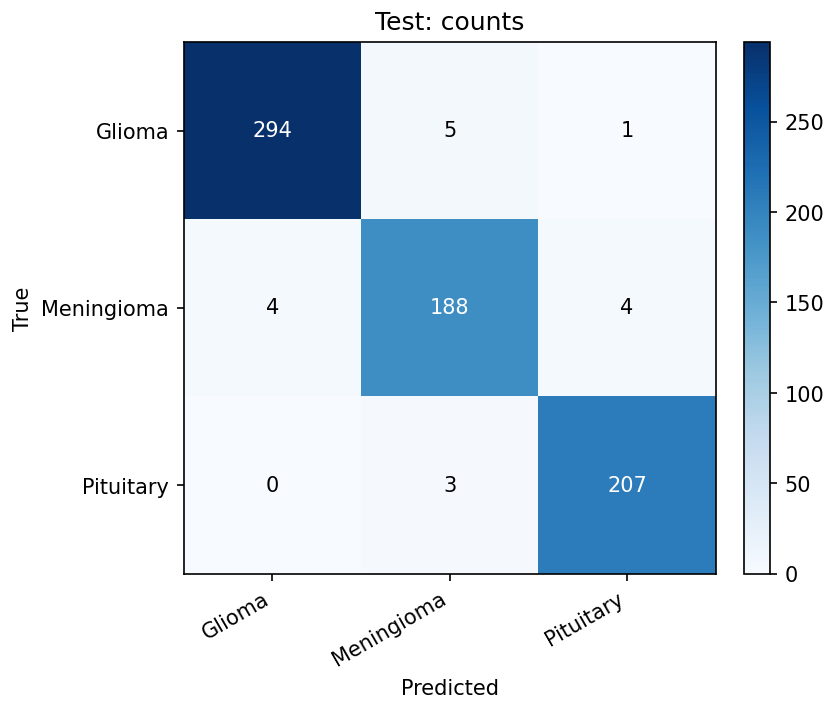
\includegraphics[width=0.62\linewidth]{figures/cls_confusion_test.png}
\caption{Test-split confusion matrix for \textbf{EfficientNetB0} on the multiclass classification task, with 17 errors in total. Most residual confusion occurs between meningioma and the other two classes. Validation and row-normalised panels are given in Supplementary Figure~S14.}
\label{fig:cls-confusion}
\end{figure}

\subsection{Model Efficiency Comparison}
\label{sec:efficiency}

Table~\ref{tab:efficiency} compares computational cost for both tasks in paired columns, with all measurements taken on the same Tesla T4 hardware; the complete per-task measurements, including batch size and training time, are given in Supplementary Tables~S9 and S10. Three distinct efficiency regimes are visible. The lightweight CNNs, EfficientNetB0 and MobileNetV3-Large, require under 0.8 GFLOPs per image and deliver the highest batched throughput, at 1,364 and 2,409 images per second respectively on the binary task. The mid-sized convolutional and hybrid models, DenseNet121, ResNet50, InceptionV3, and CoAtNet-0, occupy an intermediate band of 5.7 to 11.4 GFLOPs. The InceptionV3 figure of 11.42 GFLOPs is not like-for-like with the others, because it is computed at the native InceptionV3 input of $299\times 299$ pixels rather than the $224\times 224$ pixels used by every other model; with 1.78 times as many input pixels, its cost per image is inflated relative to the rest of the band, and its position at the top of that band reflects input resolution as well as architecture. The large transformers and VGG16 sit at 22.5 to 30.9 GFLOPs and deliver the lowest throughput, with Swin-Base managing only 196 images per second on the binary task, roughly one twelfth of MobileNetV3-Large.

The accuracy-per-million-parameters columns make the architectural efficiency difference stark. On the binary task EfficientNetB0 achieves 24.79 percentage points of accuracy per million parameters, MobileNetV3-Large 21.60, and DenseNet121 14.29, while the transformers deliver 1.11 and VGG16 only 0.66; EfficientNetB0 is therefore more than thirty-seven times more parameter-efficient than VGG16 while also being eleven percentage points more accurate, and on the multiclass task it again leads at 24.33 points per million, more than twenty times the figure for either transformer. Wall-clock training time does not track parameter count, because batch size, input resolution, and attention cost all intervene: CoAtNet-0 required 29.1 minutes for the binary task while EfficientNetB0 required 16.3 minutes despite being the smallest model in the study, a consequence of CoAtNet-0 running at batch size 64 against 256 and therefore taking four times as many optimiser steps (Supplementary Table~S9). The binary InceptionV3 training time of 4.9 minutes should be disregarded for comparison purposes: as described in Section~\ref{sec:impl}, that run executed on a single GPU rather than two, so its wall-clock figure is not measured under the same conditions as the other eight rows. Its parameter count, GFLOPs, latency, and throughput are unaffected, since those were measured separately on one device for every model.

Single-image latency was measured on one Tesla T4 at batch size one under half-precision autocasting, using a synthetic input at each model's native resolution, and is reported as the mean $\pm$ standard deviation of 100 timed forward passes that followed 10 untimed warm-up passes, with the device synchronised before each timing was read. Throughput is the mean over 20 timed forward passes at batch size 32 that followed 3 warm-up passes; the per-pass timings of this batched benchmark were not retained, so no variance can be reported for throughput. Within-run standard deviations of latency range from 0.5 to 2.6~ms. They capture timing jitter within one session only: the two independent measurements of the EfficientNetB0 backbone, one per task, differ by 3.1~ms ($10.8\pm 0.5$ against $13.9\pm 1.0$~ms), well beyond either standard deviation, so latency differences of a few milliseconds between models should not be over-interpreted. With that caveat, single-image latency favours ResNet50 at $7.3\pm 0.5$~ms over EfficientNetB0 at $10.8\pm 0.5$~ms on the binary task, because the depth-wise separable convolutions that make EfficientNetB0 parameter-efficient do not map as efficiently onto the GPU at batch size one. Latency also separates the two transformers sharply despite their near-identical size: on the multiclass task Swin-Base requires $35.1\pm 2.6$~ms against $8.4\pm 0.6$~ms for ViT-B/16, because the shifted-window attention that gives Swin-Base its accuracy advantage also introduces sequential windowing operations that do not parallelise well at batch size one. Swin-Base therefore buys its leading accuracy at roughly four times the per-request latency of ViT-B/16 and more than twice that of EfficientNetB0. For deployment, the correct efficiency metric depends on whether the constraint is memory footprint, batch throughput, or single-request latency.

\begin{table*}[htbp]
\centering
\caption{Computational efficiency for the binary (Bin.) and multiclass (Multi.) tasks in paired columns. Latency is the mean $\pm$ standard deviation of 100 timed single-image forward passes after 10 warm-up passes; ``Thr.'' is throughput in images per second at batch size 32, averaged over 20 timed passes; ``Acc./M'' is test accuracy in percentage points per million parameters. All inference measurements used one Tesla T4 under half-precision autocasting. A dash marks a model not run on the multiclass task. Batch sizes and training times are given in Supplementary Tables~S9 and S10. Rows are ordered by parameter count.}
\label{tab:efficiency}
\small
\begin{tabular*}{\textwidth}{@{\extracolsep{\fill}}lcccccccc@{}}
\toprule
 & & & \multicolumn{2}{c}{Latency (ms)} & \multicolumn{2}{c}{Thr. (img/s)} & \multicolumn{2}{c}{Acc./M} \\
\cmidrule(lr){4-5}\cmidrule(lr){6-7}\cmidrule(l){8-9}
Model & Params (M)$^{a}$ & GFLOPs & Bin. & Multi. & Bin. & Multi. & Bin. & Multi. \\
\midrule
EfficientNetB0 & 4.01 & 0.77 & $10.8\pm 0.5$ & $13.9\pm 1.0$ & 1364 & 1471 & 24.79 & 24.33 \\
MobileNetV3-Large & 4.20 & 0.43 & $8.1\pm 0.6$ & -- & 2409 & -- & 21.60 & -- \\
DenseNet121 & 6.95 & 5.67 & $19.4\pm 0.9$ & -- & 630 & -- & 14.29 & -- \\
ResNet50 & 23.51 & 8.17 & $7.3\pm 0.5$ & $7.8\pm 1.3$ & 771 & 792 & 4.23 & 4.15 \\
InceptionV3 & 24.35 & 11.42$^{b}$ & $14.0\pm 1.0$ & $14.2\pm 0.9$ & 514 & 533 & 4.06 & 3.91 \\
CoAtNet-0 & 26.67 & 8.42 & $13.9\pm 0.7$ & $13.2\pm 0.6$ & 520 & 499 & 3.73 & 3.69 \\
ViT-B/16 & 85.80 & 22.54 & $8.8\pm 0.6$ & $8.4\pm 0.6$ & 287 & 290 & 1.11 & 1.05 \\
Swin-Base & 86.74 & 30.86 & $29.0\pm 1.1$ & $35.1\pm 2.6$ & 196 & 202 & 1.11 & 1.14 \\
VGG16 & 134.26 & 30.93 & $8.2\pm 0.5$ & -- & 338 & -- & 0.66 & -- \\
\bottomrule
\multicolumn{9}{@{}l}{\footnotesize $^{a}$Binary models; the multiclass InceptionV3 and Swin-Base models measure 25.12 and 86.75 million parameters (Section~\ref{sec:impl}).} \\
\multicolumn{9}{@{}l}{\footnotesize $^{b}$Computed at the native $299\times 299$ input; every other model is measured at $224\times 224$, so this value is not like-for-like.}
\end{tabular*}
\end{table*}

Calibration quality, reported in Table~\ref{tab:calibration}, adds a dimension that accuracy alone does not capture. The four leading binary models are all well calibrated, with expected calibration errors between 0.0044 and 0.0084, meaning that a predicted confidence of 95\% corresponds closely to a 95\% empirical success rate. MobileNetV3-Large and VGG16, by contrast, show calibration errors of 0.0685 and 0.0437, an order of magnitude worse. This matters for deployment: a model whose confidence scores are unreliable cannot safely be used to triage cases by confidence or to defer uncertain cases to a human reader, even if its ranking performance measured by AUC appears strong. On the multiclass task all six models are reasonably calibrated, with Swin-Base best at 0.0076 and ViT-B/16 worst at 0.0266.

\begin{table}[htbp]
\centering
\caption{Expected calibration error (ECE), Matthews correlation coefficient (MCC), and Cohen's kappa on the held-out test split for both tasks. Lower ECE indicates better agreement between predicted confidence and observed accuracy.}
\label{tab:calibration}
\small
\begin{tabular*}{\textwidth}{@{\extracolsep{\fill}}llccc@{}}
\toprule
Task & Model & ECE & MCC & Kappa \\
\midrule
\multirow{9}{*}{Binary}
 & DenseNet121 & 0.0044 & 0.9878 & 0.9877 \\
 & EfficientNetB0 & 0.0049 & 0.9878 & 0.9877 \\
 & ResNet50 & 0.0057 & 0.9878 & 0.9877 \\
 & InceptionV3 & 0.0078 & 0.9755 & 0.9754 \\
 & CoAtNet-0 & 0.0084 & 0.9878 & 0.9877 \\
 & Swin-Base & 0.0235 & 0.9192 & 0.9181 \\
 & ViT-B/16 & 0.0323 & 0.8978 & 0.8975 \\
 & VGG16 & 0.0437 & 0.7673 & 0.7665 \\
 & MobileNetV3-Large & 0.0685 & 0.8302 & 0.8161 \\
\midrule
\multirow{6}{*}{Multiclass}
 & Swin-Base & 0.0076 & 0.9784 & 0.9783 \\
 & InceptionV3 & 0.0077 & 0.9741 & 0.9740 \\
 & CoAtNet-0 & 0.0084 & 0.9762 & 0.9761 \\
 & EfficientNetB0 & 0.0112 & 0.9632 & 0.9632 \\
 & ResNet50 & 0.0116 & 0.9633 & 0.9632 \\
 & ViT-B/16 & 0.0266 & 0.8550 & 0.8550 \\
\bottomrule
\end{tabular*}
\end{table}

\subsection{Interpretability Results}
\label{sec:interpretability}

A performance figure alone does not establish that a model is attending to clinically relevant image regions rather than to incidental artefacts such as skull outline, field of view, or scanner-specific intensity patterns. To examine this, gradient-weighted class activation mapping was applied to EfficientNetB0 for both tasks and to Swin-Base for the multiclass task. In every case the gradients of the predicted class score with respect to the target-layer activations were averaged spatially to give one weight per channel, the weighted sum of the activations was passed through a rectified linear unit, upsampled bilinearly to the input resolution, and min--max normalised. For EfficientNetB0 the target layer is the final convolutional stage. The transformer backbones require a further choice that materially changes the resulting map. For Swin-Base the target is the first layer normalisation of the last block of the final stage; its output is already a $7\times 7$ spatial grid in channels-last order, so the only transform applied is a permutation to channels-first order. For ViT-B/16 the target is the first layer normalisation of the last encoder block, whose output is a token sequence; the class token is discarded and the remaining 196 patch tokens are reshaped to a $14\times 14$ grid before the map is computed. No attention-native method such as attention rollout was applied to corroborate the transformer maps. Two caveats therefore apply before any comparison is made. First, the activation maps of convolutional and attention stages are not strictly commensurable, because they are taken from layers of different kinds and spatial resolution, so contrasts between EfficientNetB0 and Swin-Base below are prompts for further investigation rather than measured differences. Second, the transformer maps depend on the target layer chosen, and a different layer could yield a different map.

Figure~\ref{fig:gradcam-effnet} shows the EfficientNetB0 maps for the most confident correctly classified test cases of both tasks; the full input, activation, and overlay panels are given in Supplementary Figure~S15. For correctly classified tumour-positive cases, the activation consistently concentrates on the lesion itself rather than on peripheral anatomy, which supports the interpretation that the model has learned a tumour-relevant representation for this backbone. For correctly classified tumour-negative cases the activation covers essentially the whole brain; this is the expected behaviour for a negative class, since there is no lesion to localise and the decision rests on the absence of a focal abnormality across the brain, and it should not be read as diffuse or unfocused attention. In the multiclass setting the attended regions are broadly consistent with the anatomical expectations for each subtype, with pituitary cases showing focused activation in the sellar region and glioma cases showing more diffuse activation across the affected hemisphere.

Figure~\ref{fig:cls-swin-gradcam} shows the equivalent maps for Swin-Base on the multiclass task, and the comparison is not reassuring. For meningioma the Swin-Base heat maps sit on the visible lesion, but for glioma and pituitary they largely highlight image corners and borders lying outside the brain entirely. Since Swin-Base is the most accurate subtype classifier in this study, this is a material finding: it suggests that part of its accuracy may derive from background or acquisition cues that correlate with class rather than from tumour morphology. Such cues are plausible here because the two source collections differ in native image size and framing, as Tables~\ref{tab:provenance} and \ref{tab:image-dims} show, and because class proportions differ between them, so border artefacts could carry genuine label information without carrying any clinical meaning. This observation is qualitative and drawn from a single figure; the notebooks do not test it, and no measurement against annotated masks was performed. It nevertheless tempers the headline ranking, since a model that attains 98.58\% accuracy partly by reading image borders would not retain that accuracy on data acquired under a different protocol, and it illustrates why interpretability evidence belongs alongside accuracy rather than after it.

Maps for misclassified cases are given in Supplementary Figure~S16. The selection rule matters for their interpretation: these panels show the \emph{most confident} errors, up to six per model, ranked by the probability assigned to the wrong class, and are therefore the failures in which the model was most assured, not representative or borderline ones. For EfficientNetB0 the binary panel exhausts the available errors, since only three test images were misclassified, whereas the multiclass panel shows six of seventeen. In these high-confidence failures the activation is not noticeably less focused than in the correct cases. All of these observations are qualitative rather than a quantitative interpretability evaluation. No assessment against radiologist-annotated tumour masks was carried out, because the datasets used provide class labels only and contain no segmentation masks against which the attention maps could be scored. Quantifying attention overlap against expert annotation is identified in Section~\ref{sec:conclusion} as necessary future work.

\begin{figure*}[htbp]
\centering
\begin{subfigure}{0.62\textwidth}
\centering
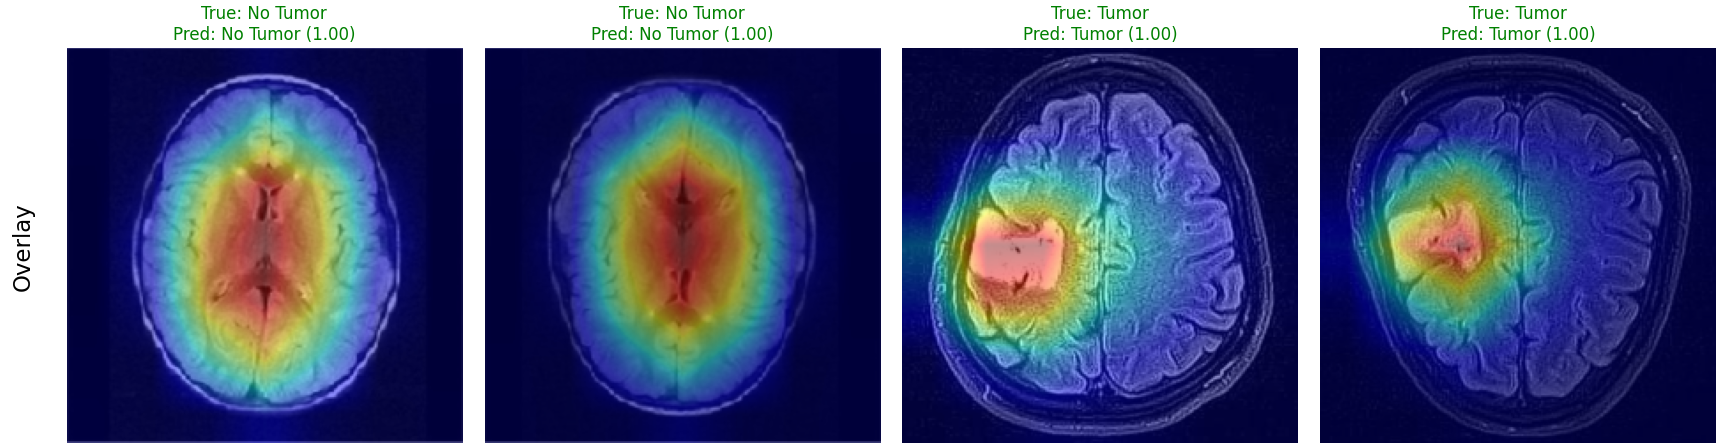
\includegraphics[width=\linewidth]{figures/binary_gradcam_correct_overlay.png}
\caption{Binary detection: two tumour-negative and two tumour-positive cases.}
\end{subfigure}
\\[4pt]
\begin{subfigure}{\textwidth}
\centering
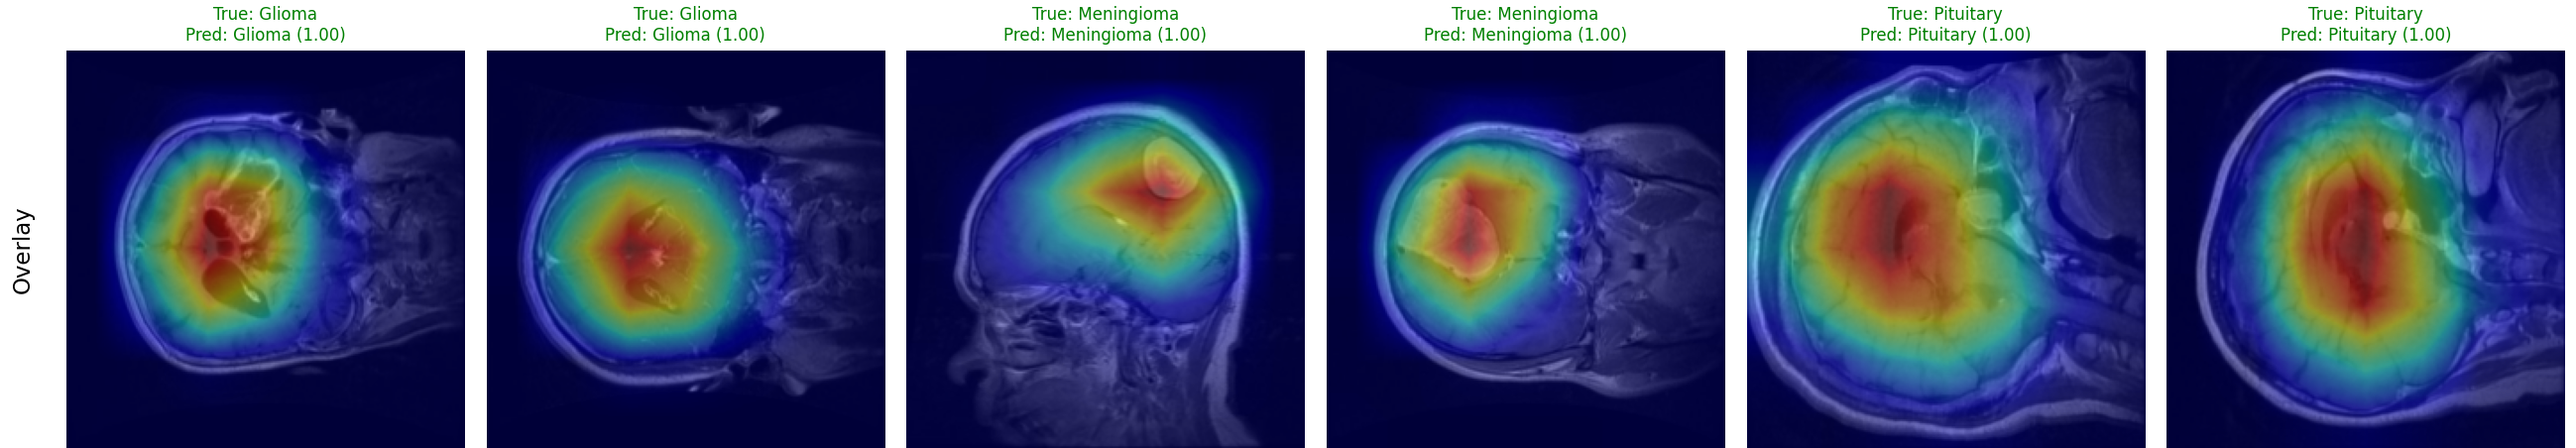
\includegraphics[width=\linewidth]{figures/cls_gradcam_correct_overlay.png}
\caption{Multiclass classification: two cases each of glioma, meningioma, and pituitary.}
\end{subfigure}
\caption{Gradient-weighted class activation maps for \textbf{EfficientNetB0}, overlaid on the most confident correctly classified test cases of each class. Activation concentrates on the lesion for tumour-positive cases and covers the whole brain for tumour-negative cases, where there is no lesion to localise. The full input, activation, and overlay panels are given in Supplementary Figure~S15.}
\label{fig:gradcam-effnet}
\end{figure*}

\begin{figure}[htbp]
\centering
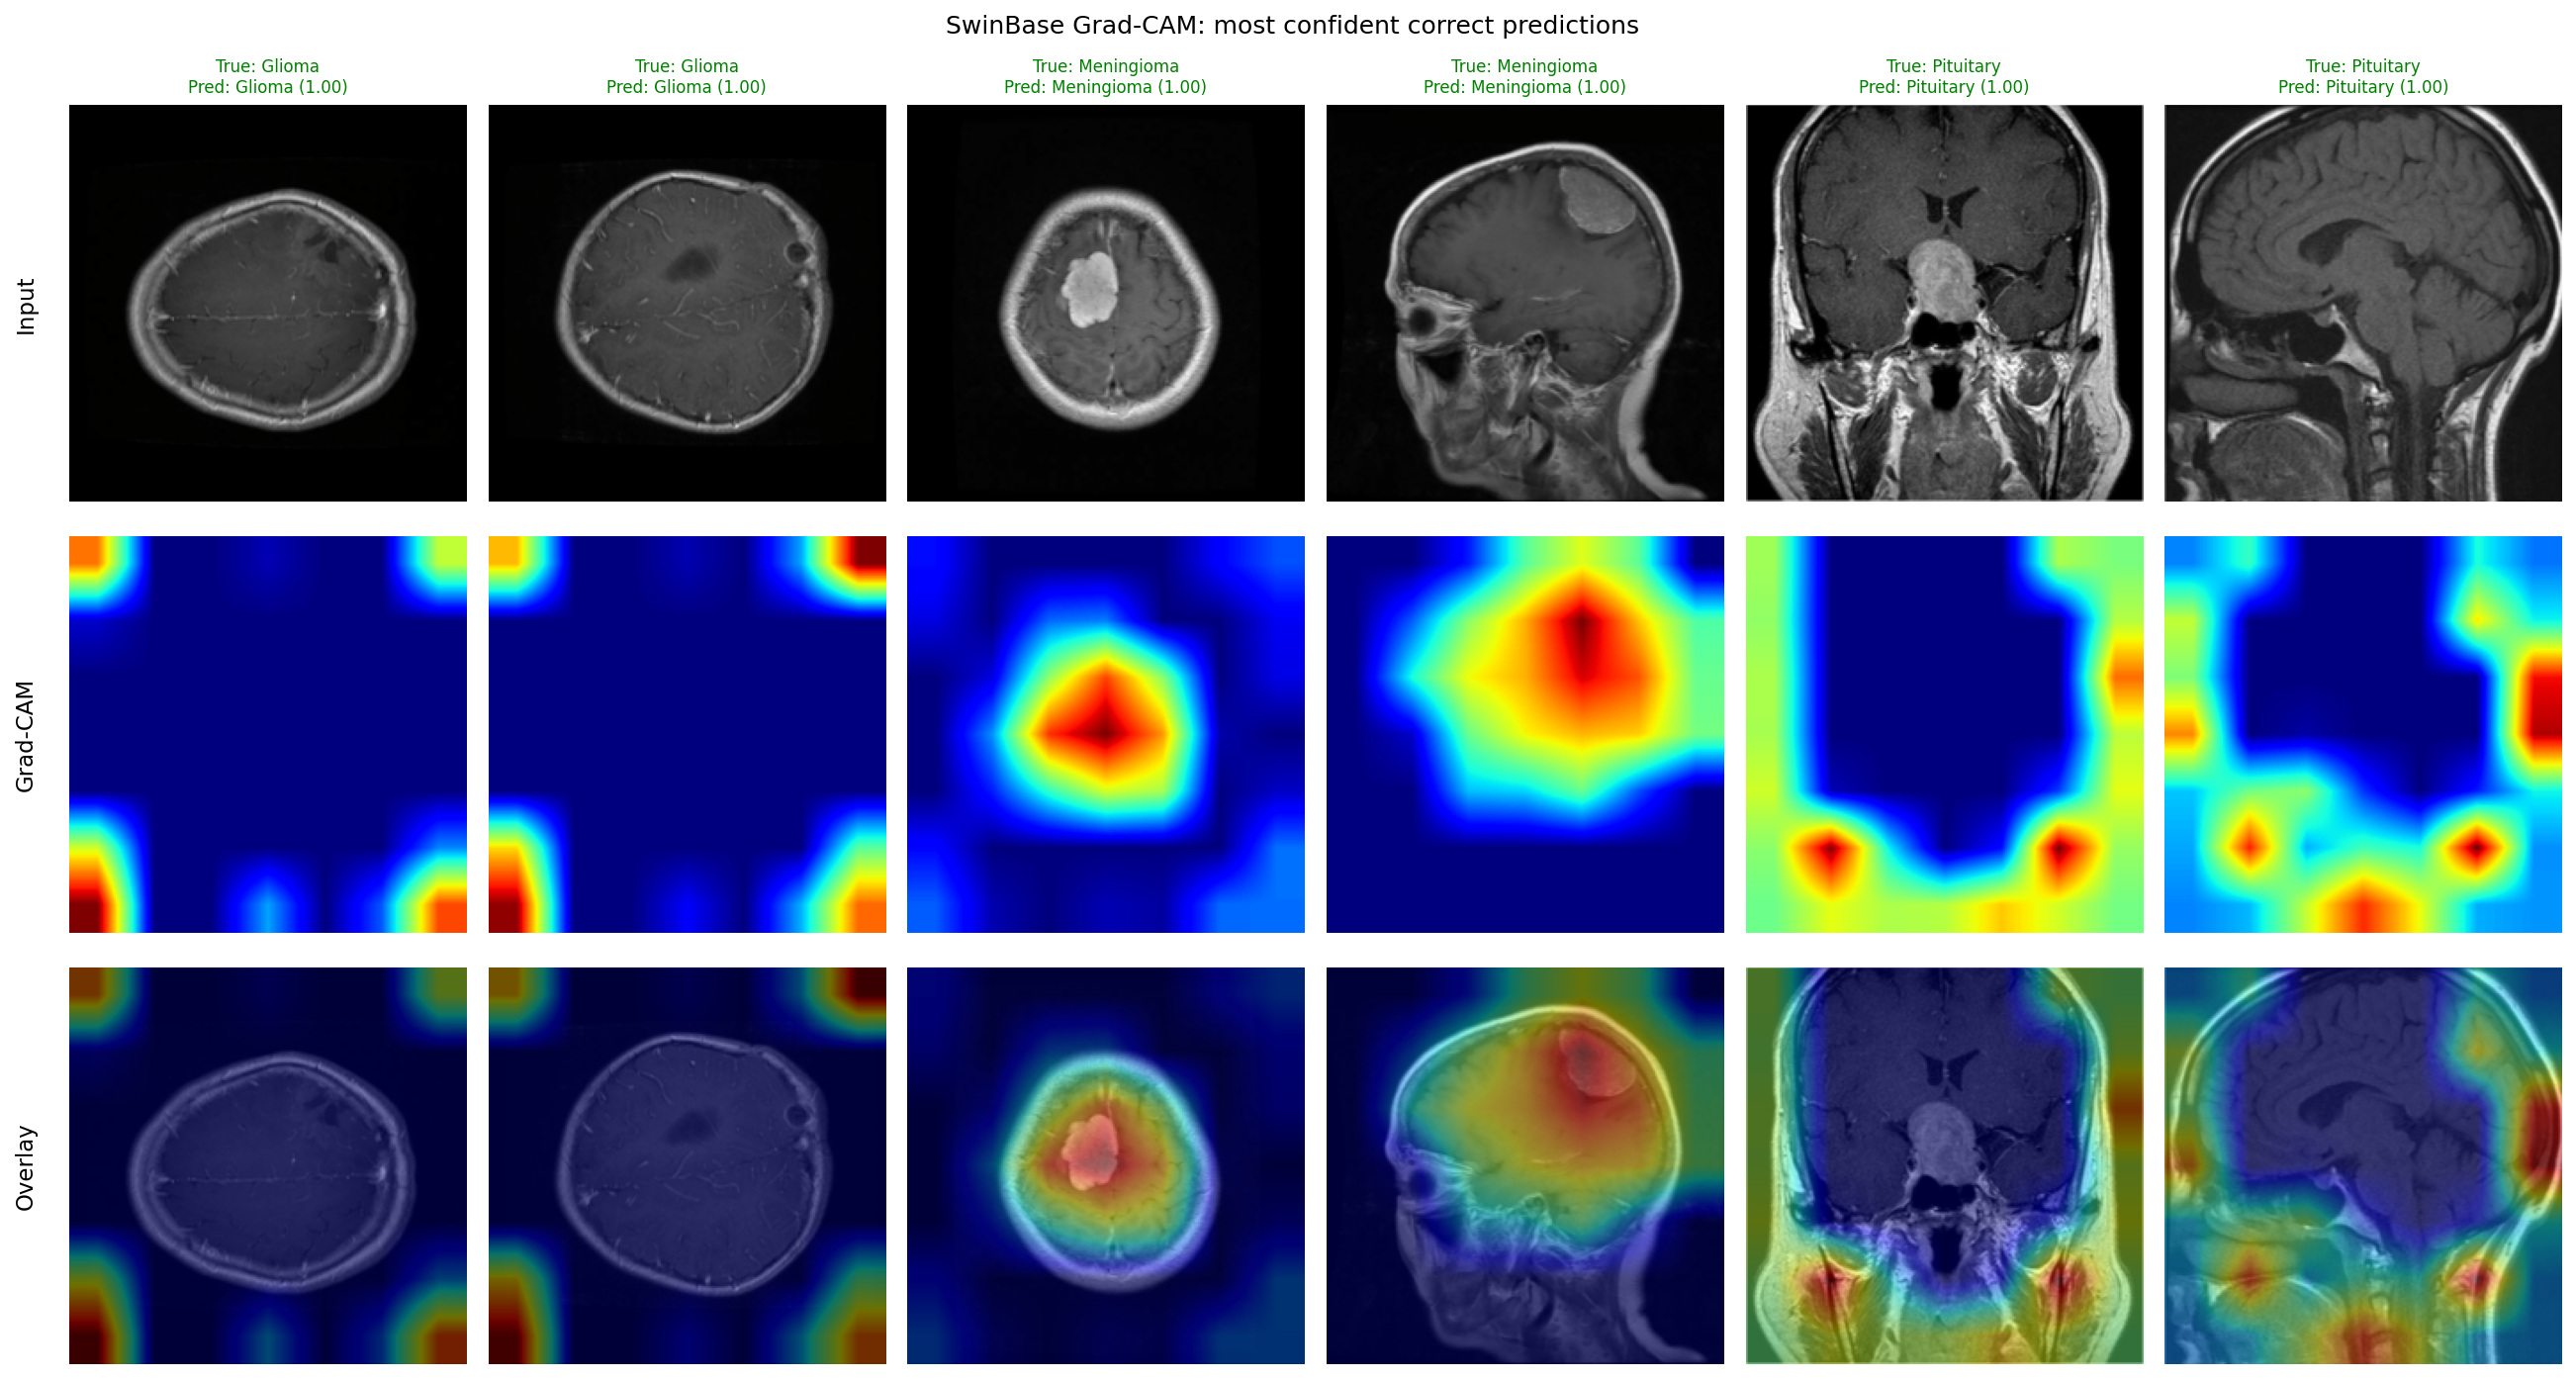
\includegraphics[width=\linewidth]{figures/cls_swin_gradcam.png}
\caption{Gradient-weighted class activation maps for \textbf{Swin-Base} on correctly classified multiclass test cases, showing the two most confident correct predictions per class. Activation sits on the lesion for meningioma but falls largely on image corners and borders outside the brain for glioma and pituitary, suggesting partial reliance on non-anatomical cues.}
\label{fig:cls-swin-gradcam}
\end{figure}

\subsection{Comparison with Existing Literature}
\label{sec:comparison}

Table~\ref{tab:literature-comparison} compares the present results with previously published studies using the same architectures. The ResNet50 and InceptionV3 results obtained here are consistent with, or exceed, the published benchmarks. Two discrepancies deserve comment. The VGG16 result of 88.32\% falls well short of the 98.69\% reported by Khan et al. \cite{ref23}; this is attributable to differences in preprocessing, augmentation strategy, and train-test partitioning, and in particular to the fact that the present protocol fixes a single shared set of hyperparameters across all nine models rather than tuning each one individually, a choice that penalises architectures such as VGG16 that are sensitive to learning rate. The DenseNet121 result of 99.39\% is marginally below the 99.51\% reported by Noreen et al. \cite{ref24}, a difference of less than one image on a test set of this size and therefore not meaningful.

More generally, direct comparison with published figures should be treated with caution, for three reasons. First, most of the studies in Table~\ref{tab:literature-comparison} evaluate on the 3,064-image Cheng collection without deduplication, whereas the multiclass results reported here are computed after removing 19.3\% of the images as near-duplicates; deduplication removes exactly the images most likely to have inflated a reported score, so a slightly lower number obtained on a deduplicated split is not evidence of a weaker model. Second, as noted in Section~\ref{sec:impl}, the multiclass pool here merges the original training and testing folders of the Bhuvaji dataset before drawing fresh stratified splits, so the test set used in this work is not the test set used by studies that adopt that dataset's official partition. Third, the models compared here share a single hyperparameter configuration rather than being individually tuned. The comparison is therefore included for orientation rather than as a like-for-like benchmark, and the absolute figures in the final column should not be cited as head-to-head wins or losses against the referenced studies.

\begin{table*}[htbp]
\centering
\caption{Comparison of the present results with previously published studies. Results obtained in this work are measured on the held-out test split.}
\label{tab:literature-comparison}
\small
\begin{tabular*}{\textwidth}{@{\extracolsep{\fill}}llcccc@{}}
\toprule
Study & Model & Dataset size & Task & Reported accuracy & This work \\
\midrule
Talo et al. (2019) \cite{ref16} & ResNet50 & 253 & Binary & 95.23\% & 99.39\% \\
Khan et al. (2020) \cite{ref23} & VGG16 & 3,064 & Binary & 98.69\% & 88.32\% \\
Noreen et al. (2020) \cite{ref24} & DenseNet121 & 3,064 & Binary & 99.51\% & 99.39\% \\
Rehman et al. (2020) \cite{ref25} & InceptionV3 & 3,064 & Binary & 99.34\% & 98.77\% \\
Deepak and Ameer (2019) \cite{ref15} & InceptionV3 & 3,064 & Multiclass & 97.50\% & 98.30\% \\
\bottomrule
\end{tabular*}
\end{table*}

Several architectural innovations contribute to improved performance in medical imaging tasks. Residual learning in ResNet enables the training of deeper networks that capture hierarchical representations from low-level edges to high-level semantic features. Dense connections maximise information flow and feature reuse with comparatively few parameters, which explains why DenseNet121 matches the accuracy of ResNet50 with less than a third of its parameters. Inception modules capture tumours of varying size through parallel convolutional paths of different kernel sizes. Attention mechanisms in CoAtNet-0 and Swin-Base model long-range dependencies that are relevant for relating a tumour region to surrounding healthy tissue. Neural architecture search in EfficientNetB0 and MobileNetV3-Large optimises architectural decisions beyond human intuition, though the MobileNetV3-Large result shows that architectural efficiency does not by itself guarantee stable optimisation under a fixed shared training budget.

The clearest cross-cutting finding is what may be termed the transformer paradox: pure transformers underperformed while hybrid convolution-attention models excelled. ViT-B/16 was the weakest model on both tasks despite being among the largest, whereas CoAtNet-0 was among the strongest on both. With training sets of 2,277 and 3,293 images, there is insufficient data for a pure transformer to learn the spatial inductive biases that convolutional architectures encode by construction. The practical implication for medical imaging at this data scale is that attention should be adopted in hybrid form rather than in isolation.

Regarding model selection, the appropriate choice depends on the deployment constraint. Where accuracy is the primary consideration and computational resources are not limiting, Swin-Base is the strongest subtype classifier at 98.58\% accuracy, and CoAtNet-0 offers almost the same accuracy at 98.44\% for less than a third of the parameters and a threefold higher throughput. Where deployment is on constrained hardware, EfficientNetB0 is the clear recommendation: it reaches 99.39\% detection accuracy and 97.59\% subtype accuracy with 4.01 million parameters, 0.77 GFLOPs per image, and well-calibrated confidence scores. Where single-request latency dominates, ResNet50 provides the fastest single-image inference at $7.3\pm 0.5$~ms while retaining 99.39\% detection accuracy, and it remains a reasonable default baseline for further research. No single model dominates on every axis, and the evidence presented here is intended to support a selection made against explicit deployment requirements.

The misclassification panels of Section~\ref{sec:interpretability} carry a further implication for deployment. They show the most confident errors, and in those errors the activation maps are as plausible-looking as in correct predictions. Confidently wrong predictions with plausible-looking attention maps cannot be filtered by confidence thresholding, because the confidence is high, or by visual review of the map, because the map looks reasonable. This is a direct argument against deploying Grad-CAM as a clinical safety check: an explanation map can accompany a prediction, but it cannot be relied on to flag the predictions that are wrong.

\section{Conclusion}
\label{sec:conclusion}

This study benchmarked nine ImageNet-pretrained architectures for brain tumour detection, and six of them for subtype classification, under matched data, preprocessing, and training schedule, with perceptual-hash deduplication removing 19.3\% of the multiclass images before splitting. On binary detection, CoAtNet-0, DenseNet121, EfficientNetB0, and ResNet50 each reached 99.39\% test accuracy and are statistically indistinguishable, while MobileNetV3-Large at 90.78\% and VGG16 at 88.32\% proved inadequate. On subtype classification, Swin-Base led at 98.58\%, followed by CoAtNet-0 at 98.44\% and InceptionV3 at 98.30\%, with EfficientNetB0 and ResNet50 at 97.59\% and ViT-B/16 trailing at 90.51\%.

Three findings carry beyond the leaderboard. First, the hybrid CoAtNet-0 consistently outperformed the pure transformer ViT-B/16 of three times its size, indicating that at this data scale attention should be paired with a convolutional prior. Second, parameter efficiency and accuracy are not in tension: EfficientNetB0 matched or approached far larger models with 4.01 million parameters and 0.77 GFLOPs per image. Third, headline accuracy conceals clinically material differences: models with identical accuracy differed in whether their errors were missed tumours or false alarms, MobileNetV3-Large combined a strong AUC with poor calibration, and the Grad-CAM evidence indicates that the most accurate subtype model attends partly to regions outside the brain, so accuracy alone does not establish that pathology has been learned.

The principal limitations are as follows. The datasets are public two-dimensional slice collections of unknown MRI sequence composition, the binary negative class is tumour-negative rather than certified normal, and no external validation was performed. Each model was trained once for ten epochs with a single shared configuration, and batch size varied from 32 to 256, so the optimisation budget is uncontrolled and the leading models cannot be separated statistically. Deduplication was applied to the multiclass track only, by an order-dependent procedure that resolves cross-class near-duplicates in favour of glioma without counting them, and splits were drawn at slice rather than patient level. Swin-Base was sourced from different implementations in the two tasks, and the interpretability evidence is qualitative.

Future work should apply the same deduplication to the binary track and make it label-aware, reporting cross-label collisions and sensitivity to the Hamming threshold; split by patient where identifiers are available; equalise the optimisation budget by fixing the number of gradient updates; adopt repeated runs with cross-validation; quantify the fraction of Grad-CAM energy falling outside the brain and test for shortcut learning with background-only ablation; and validate externally on multi-sequence and three-dimensional institutional data before any clinical claim is made. The architectures examined here are accurate enough to warrant investigation as second-reader aids rather than autonomous diagnostics, and the accompanying code and per-model artefacts are released so that both the results and their caveats can be reproduced and extended.

\section*{Declaration of competing interest}

The authors declare that they have no known competing financial interests or personal relationships that could have appeared to influence the work reported in this paper.

\section*{Data availability}

All datasets used in this study are publicly available and are cited in Section~\ref{sec:data}. The complete code, trained model checkpoints, and per-model evaluation artefacts are available at the repository given in \ref{app:code}.

\section*{Supplementary material}

Supplementary material associated with this article is provided in a separate file. It contains the per-class detection and classification metrics (Supplementary Tables~S4 and S5), the training and validation metrics at the checkpointed epoch (Supplementary Tables~S6 and S7), the complete efficiency measurements for each task (Supplementary Tables~S9 and S10), and Supplementary Figures~S1--S16, covering dataset characterisation, augmentation, training curves, receiver operating characteristic, precision--recall and reliability curves for every model, per-class and prediction summaries, full confusion panels, and the complete gradient-weighted class activation maps for correct and misclassified cases.

\begin{thebibliography}{99}

\bibitem{ref1} E. I. Zacharaki, S. Wang, S. Chawla, et al., ``Classification of brain tumor type and grade using MRI texture and shape in a machine learning scheme,'' Magnetic Resonance in Medicine, vol. 62, no. 6, pp. 1609-1618, 2009.

\bibitem{ref2} S. Bauer, R. Wiest, L. P. Nolte, and M. Reyes, ``A survey of MRI-based medical image analysis for brain tumor studies,'' Physics in Medicine and Biology, vol. 58, no. 13, pp. R97-R129, 2013.

\bibitem{ref3} N. Gordillo, E. Montseny, and P. Sobrevilla, ``State of the art survey on MRI brain tumor segmentation,'' Magnetic Resonance Imaging, vol. 31, no. 8, pp. 1426-1438, 2013.

\bibitem{ref4} K. Simonyan and A. Zisserman, ``Very deep convolutional networks for large-scale image recognition,'' arXiv preprint arXiv:1409.1556, 2014.

\bibitem{ref5} J. Cheng, W. Huang, S. Cao, et al., ``Enhanced performance of brain tumor classification via tumor region augmentation and partition,'' PLoS ONE, vol. 10, no. 10, p. e0140381, 2015.

\bibitem{ref6} K. He, X. Zhang, S. Ren, and J. Sun, ``Deep residual learning for image recognition,'' in Proc. IEEE Conf. Comput. Vis. Pattern Recognit. (CVPR), 2016, pp. 770-778.

\bibitem{ref7} C. Szegedy, V. Vanhoucke, S. Ioffe, J. Shlens, and Z. Wojna, ``Rethinking the inception architecture for computer vision,'' in Proc. IEEE Conf. Comput. Vis. Pattern Recognit. (CVPR), 2016, pp. 2818-2826.

\bibitem{ref9} G. Huang, Z. Liu, L. Van Der Maaten, and K. Q. Weinberger, ``Densely connected convolutional networks,'' in Proc. IEEE Conf. Comput. Vis. Pattern Recognit. (CVPR), 2017, pp. 4700-4708.

\bibitem{ref12} J. Seetha and S. S. Raja, ``Brain tumor classification using convolutional neural networks,'' Biomedical and Pharmacology Journal, vol. 11, no. 3, p. 1457, 2018.

\bibitem{ref13} A. L. Beam and I. S. Kohane, ``Big data and machine learning in health care,'' JAMA, vol. 319, no. 13, pp. 1317-1318, 2018.

\bibitem{ref14} J. De Fauw, J. R. Ledsam, B. Romera-Paredes, et al., ``Clinically applicable deep learning for diagnosis and referral in retinal disease,'' Nature Medicine, vol. 24, no. 9, pp. 1342-1350, 2018.

\bibitem{ref15} S. Deepak and P. M. Ameer, ``Brain tumor classification using deep CNN features via transfer learning,'' Computers in Biology and Medicine, vol. 111, p. 103345, 2019.

\bibitem{ref16} M. Talo, U. B. Baloglu, \"O. Y{\i}ld{\i}r{\i}m, and U. R. Acharya, ``Application of deep transfer learning for automated brain abnormality classification using MR images,'' Cognitive Systems Research, vol. 54, pp. 176-188, 2019.

\bibitem{ref18} M. Tan and Q. Le, ``EfficientNet: Rethinking model scaling for convolutional neural networks,'' in Proc. Int. Conf. Mach. Learn. (ICML), 2019, pp. 6105-6114.

\bibitem{ref19} A. Howard, M. Sandler, G. Chu, et al., ``Searching for MobileNetV3,'' in Proc. IEEE/CVF Int. Conf. Comput. Vis. (ICCV), 2019, pp. 1314-1324.

\bibitem{ref23} M. A. Khan, I. Ashraf, M. Alhaisoni, et al., ``Multimodal brain tumor classification using deep learning and robust feature selection: A machine learning application for radiologists,'' Diagnostics, vol. 10, no. 8, p. 565, 2020.

\bibitem{ref24} N. Noreen, S. Palaniappan, A. Qayyum, I. Ahmad, M. Imran, and M. Shoaib, ``A deep learning model based on concatenation approach for the diagnosis of brain tumor,'' IEEE Access, vol. 8, pp. 55135-55144, 2020.

\bibitem{ref25} A. Rehman, S. Naz, M. I. Razzak, F. Akram, and M. Imran, ``A deep learning-based framework for automatic brain tumors classification using transfer learning,'' Circuits, Systems, and Signal Processing, vol. 39, no. 2, pp. 757-775, 2020.

\bibitem{ref26} N. Ghassemi, A. Shoeibi, and M. Rouhani, ``Deep neural network with generative adversarial networks pre-training for brain tumor classification based on MR images,'' Biomedical Signal Processing and Control, vol. 57, p. 101678, 2020.

\bibitem{ref28} A. Dosovitskiy, L. Beyer, A. Kolesnikov, et al., ``An image is worth 16x16 words: Transformers for image recognition at scale,'' in Proc. Int. Conf. Learn. Represent. (ICLR), 2021.

\bibitem{ref29} Z. Liu, Y. Lin, Y. Cao, et al., ``Swin transformer: Hierarchical vision transformer using shifted windows,'' in Proc. IEEE/CVF Int. Conf. Comput. Vis. (ICCV), 2021, pp. 10012-10022.

\bibitem{ref30} Z. Dai, H. Liu, Q. V. Le, and M. Tan, ``CoAtNet: Marrying convolution and attention for all data sizes,'' in Advances in Neural Information Processing Systems (NeurIPS), vol. 34, 2021, pp. 3965-3977.

\bibitem{ref32} S. Khan, M. Naseer, M. Hayat, S. W. Zamir, F. S. Khan, and M. Shah, ``Transformers in vision: A survey,'' ACM Computing Surveys, vol. 54, no. 10s, pp. 1-41, 2022.

\bibitem{cbtrus} Q. T. Ostrom, M. Price, C. Neff, et al., ``CBTRUS statistical report: Primary brain and other central nervous system tumors diagnosed in the United States in 2016--2020,'' Neuro-Oncology, vol. 25, suppl. 4, pp. iv1-iv99, 2023, doi: \url{https://doi.org/10.1093/neuonc/noad149}

\bibitem{tummala2022} S. Tummala, S. Kadry, S. A. C. Bukhari, and H. T. Rauf, ``Classification of brain tumor from magnetic resonance imaging using vision transformers ensembling,'' Current Oncology, vol. 29, no. 10, pp. 7498-7511, 2022, doi: \url{https://doi.org/10.3390/curroncol29100590}

\bibitem{asiri2024} A. A. Asiri, A. Shaf, T. Ali, et al., ``Advancing brain tumor detection: Harnessing the Swin Transformer's power for accurate classification and performance analysis,'' PeerJ Computer Science, vol. 10, p. e1867, 2024, doi: \url{https://doi.org/10.7717/peerj-cs.1867}

\bibitem{shamshad2023} F. Shamshad, S. Khan, S. W. Zamir, et al., ``Transformers in medical imaging: A survey,'' Medical Image Analysis, vol. 88, p. 102802, 2023, doi: \url{https://doi.org/10.1016/j.media.2023.102802}

\bibitem{kapoor2023} S. Kapoor and A. Narayanan, ``Leakage and the reproducibility crisis in machine-learning-based science,'' Patterns, p. 100804, 2023, doi: \url{https://doi.org/10.1016/j.patter.2023.100804}

\bibitem{vangala2026} B. P. Vangala, S. Guda, L. Peddi, and N. Vangala, ``Scores that hold, benchmarks that leak: Measuring dataset contamination in public brain-tumor MRI classification,'' arXiv preprint arXiv:2610.00421, 2026.

\bibitem{ds1} N. Chakrabarty, ``Brain MRI images for brain tumor detection,'' Kaggle dataset, version 1, 2019. [Online]. Available: \url{https://www.kaggle.com/datasets/navoneel/brain-mri-images-for-brain-tumor-detection}

\bibitem{ds2} A. Hamada, ``Br35H :: Brain tumor detection 2020,'' IEEE DataPort, 2025, doi: \url{https://doi.org/10.21227/tbkk-q937}. Also available on Kaggle: \url{https://www.kaggle.com/datasets/ahmedhamada0/brain-tumor-detection}

\bibitem{ds3} S. Bhuvaji, A. Kadam, P. Bhumkar, S. Dedge, and S. Kanchan, ``Brain tumor classification (MRI),'' Kaggle dataset, 2020, doi: \url{https://doi.org/10.34740/KAGGLE/DSV/1183165}

\bibitem{ds4} J. Cheng, ``Brain tumor dataset,'' figshare, version 5, 2017, doi: \url{https://doi.org/10.6084/m9.figshare.1512427.v5}

\bibitem{ds5} MoundirB, ``Jun Cheng brain tumor MRI dataset JPG,'' Kaggle dataset, version 1, 2025. JPEG conversion of \cite{ds4}. [Online]. Available: \url{https://www.kaggle.com/datasets/moundir8/jun-cheng-brain-tumor-mri-dataset-jpg}

\end{thebibliography}

\FloatBarrier
\appendix

\section{Code Repository}
\label{app:code}

The complete code for all experiments, including data preprocessing, perceptual hash deduplication, model training, evaluation, and figure generation, together with the trained checkpoints and the full per-model metric artefacts, is available at \url{https://github.com/parthmital/NeuroScan-AI}.

\end{document}
